%%
% 今時jarticleやjbook使ってる人いる?時代はjsarticleかjsbookだよ
% ついでに言うと、uplatexってのはplatexの上位互換、これを使わないなんて旧世代だよね
%
\documentclass[uplatex, report, a4j, 10pt]{jsbook}


%%
% パッケージ群
%
\usepackage{miyazaki-u-paper}   % 宮崎大学工学部の卒論の基本(片山先生作)を、僕がちょっと書き換えちゃった(テヘッ
\usepackage{enumitem}           % enumerate?古い古い
\usepackage[dvipdfmx]{graphicx,hyperref} % 当然dvipdfmなんて使ってないよね
\usepackage{graphicx}
\usepackage[dvipdfmx]{color}    % listingsを使うときにはこれも必須、dvipdfmxを変えちゃうとgraphicxのdvipdfmxも変わるよ
\usepackage{pxjahyper}
\usepackage{listings, jlisting} % コードを埋め込むなら必須
\usepackage{txfonts}            % フォントといえばやっぱりtxfonts、今はnewtxってのもあるらしい
\usepackage{verbatim}           % コメントアウトしてくれる便利なプリアンブルが使える \begin{comment} ... \end{comment}
\usepackage{url}
\usepackage{enumitem}
\usepackage{pdfpages}
% \setlistdepth{6}
% \renewlist{itemize}{itemize}{10}
\hypersetup{
setpagesize=false,
 bookmarksnumbered=true,%
 bookmarksopen=true,%
 colorlinks=true,%
 linkcolor=black,
 citecolor=black,
 filecolor=black,
 urlcolor=black,
}
% \usepackage{easy-todo}
\usepackage[hdivide={21mm, , 21mm}, vdivide={30mm, , 25mm}]{geometry} % スタイルを少し変えたくても\hoffset, \voffsetは使わないでね

% todoコマンドを追加
\newcommand\todo[1]{\PackageWarning{Todo}{Detection TODO:#1}\textcolor{red}{(TODO:#1)}}


\renewcommand{\lstlistingname}{コード}
\lstset{
  language={Java},
  frame=tlBR,%フレーム線の指定,上右下左の順,大文字は二重線
%  frameround=tttt,%角の指定,右上|右下|左下|左上の順,tは丸角,fは四角
  framesep=5pt,%本文からframeまでの間隔
  framerule=.2pt,%線の太さ
%  rulecolor={\color[gray]},%線の色
%  backgroundcolor={\color[gray]{.9}},%背景色の指定
  basicstyle={\scriptsize\ttfamily \color[gray]{.15}},%書体の指定,この場合は7ptのタイプライタ体
  identifierstyle={\ttfamily},%識別子の書体
  keywordstyle={\ttfamily \color[cmyk]{0,1,0,0}},%言語ワードの書体
  stringstyle={\scriptsize\ttfamily \color[rgb]{0,0,1}},%文字列リテラルの書体
  commentstyle={\itshape \color[cmyk]{1,0,1,0}},%コメントの書体
  numberstyle={\scriptsize},%行番号の書式
  stepnumber=1,%行番号のステップ間隔
  numbers=left,%行番号の位置
  numbersep=1em,%本文との間隔
  breaklines=true,%改行の設定
  xleftmargin=0zw,
  xrightmargin=0zw,
  columns=[l]{fullflexible},
  lineskip=-0.5zw,
  morecomment={[s][{\color[cmyk]{1,0,0,0}}]{/**}{*/}},
  floatplacement=t,
  classoffset=1,
  showstringspaces=false,%空行の表示
%  breakatwhitespace=true,
%  tabsize=5,
}

\lstdefinestyle{g4}{
  language={C},
  frame=tlBR,%フレーム線の指定,上右下左の順,大文字は二重線
%  frameround=tttt,%角の指定,右上|右下|左下|左上の順,tは丸角,fは四角
  framesep=5pt,%本文からframeまでの間隔
  framerule=.2pt,%線の太さ
%  rulecolor={\color[gray]},%線の色
%  backgroundcolor={\color[gray]{.9}},%背景色の指定
  basicstyle={\scriptsize\ttfamily \color[gray]{.15}},%書体の指定,この場合は7ptのタイプライタ体
  identifierstyle={\ttfamily},%識別子の書体
  keywordstyle={\ttfamily \color[cmyk]{0,1,0,0}},%言語ワードの書体
  stringstyle={\scriptsize\ttfamily \color[rgb]{0,0,1}},%文字列リテラルの書体
  commentstyle={\itshape \color[cmyk]{1,0,1,0}},%コメントの書体
  numberstyle={\scriptsize},%行番号の書式
  stepnumber=1,%行番号のステップ間隔
  numbers=left,%行番号の位置
  numbersep=1em,%本文との間隔
  breaklines=true,%改行の設定
  xleftmargin=0zw,
  xrightmargin=0zw,
  columns=[l]{fullflexible},
  lineskip=-0.5zw,
  morecomment={[s][{\color[cmyk]{1,0,0,0}}]{/**}{*/}},
  floatplacement=t,
  classoffset=1,
  showstringspaces=false,%空行の表示
%  breakatwhitespace=true,
%  tabsize=5,
}


% \lstset{language = modelica,
%         basicstyle=\fontsize{9pt}{10.5pt}\ttfamily,
%         backgroundcolor={\color[gray]{.90}},
%         breakindent = 10pt
%         }
%%
% miyazaki-u-paper.sty用設定値
%
\degree{g} % Graduateのg or Masterのm
\figurenumbering{f} % 図目次を付ける場合はt (真) を持つ真偽値を引数に取る関数
\tablenumbering{f} % 表目次を付ける場合はt (真) を持つ真偽値を引数に取る関数
\title{OpenModelicaのシミュレーション結果を\\用いたモータ特性表自動生成ツールの試作}
\author{原田 海人}
\nendo{元} % 年度
\advisor{片山 徹郎 教授} % 修論では無視する
\major{情報システム工学科}




\begin{document}
\maketitle


%
% 本文
%
\chapter{はじめに}\label{cha:Introduction}
近年ソフトウェア開発の効率化が求められており、設計段階や製品を試作する前に、製品の機能や性能を検証したいというニーズが高まっている\cite{modelicaモデルベース本}。
このニーズに応えるために、モデルベースシステム開発手法がある\cite{modelicaモデルベース本}。モデルベースシステム開発手法とは、製品の設計を元にシミュレーションツールを用いて、
シミュレーションを行いながら、設計品質の向上を図る開発手法である\cite{ipa_2016}。設計の品質が向上することによって、不具合が減り、手戻りを削減できるため、生産性の向上が期待できる\cite{ipa_2016}。

モデルベースシステム開発手法は、 組込みシステムの開発において特に重要である\cite{ipa_useful_modelbase_dev}。製品開発を行う際に、モデルベースシステム開発手法を適用することで、
実際に製品を試作することなく、製品の様々な性能を事前に確認できるため、開発コストを削減できる\cite{modelicaモデルベース本}。また、実際に試作品を作る回数を減らすことができるため、
製品開発の納期の短縮が期待できる。

モデルベースシステム開発手法を用いた組込みシステムの開発に、OpenModelica\cite{open_modelica}が使われる。
OpenModelicaは、Modelica\cite{modelicaモデルベース本}コードのモデリング、シミュレーション、デバッグのための機能などを持つオープンソースプラットフォームである。
OpenModelicaが出力するシミュレーションの結果は、グラフや数値であり、数値においては、csvファイルに出力できる。しかし、この出力を用いて、性能を決定付ける特定の値を確認するためには、手間と時間がかかる。
そこで、本研究では、性能を決定付ける特定の値を確認するためにかかる時間の削減を目的として、OpenModelicaのシミュレーション結果を用いたモータ特性表自動生成ツールの試作を行う。
特性表とは、製品の性能をまとめた一覧表であり、複数の製品の性能比較をする際に利用される[参考文献]。特性表を用いることで、性能の特定の値を容易に確認できるため、本研究の生成対象とする。また、本研究では、シミュレーションの対象として、ブラシ付きDCモータ[モータ使う]を対象とする。


モデルベースシステム開発手法を用いた組込みシステムの開発に、OpenModelica\cite{open_modelica}が使われる。OpenModelicaは、
Modelica\cite{modelicaモデルベース本}コードのモデリング、シミュレーション、デバッグのための機能などを持つオープンソースプラットフォームである。
OpenModelicaが出力するシミュレーションの結果は、グラフや数値であり、csvファイルに出力できる。しかし、この出力を用いて、性能を決定付ける特定の値を確認するためには、手間と時間がかかる。
そこで、本研究では、性能を決定付ける特定の値を確認するためにかかる時間の削減を目的として、OpenModelicaのシミュレーション結果を用いた特性表の自動生成ツールの試作を行う。特性表とは、製品の性能をまとめた表であり、
特性表を用いることで、特定の値を容易に確認できる。なお、本研究では、シミュレーションの対象として、ブラシ付きDCモータ\cite{モータ使う}を対象とする。

% この問題を解決する手段の1つとして、特性表を用いることが考えられる。しかし、特性表の作成は、人手により作成するため、手間と時間を必要とする。OpenModelicaのシミュレーション結果を用いて、特性表を作成するためには、OpenModelicaが出力したcsvファイルから特定の値を算出し、グラフを生成する必要がある。

本論文の構成は、以下の通りである。\\
第2章では、モータ特性表自動生成ツールを試作するために必要となる前提知識について説明する。\\
第3章では、試作したモータ特性表自動生成ツールの構成および実装について説明する。\\
第4章では、試作したモータ特性表自動生成ツールが正しく動作することを検証する。\\
第5章では、試作したモータ特性表自動生成ツールについて考察する。\\
第6章では、本論文のまとめと今後の課題を述べる。\\
\chapter{研究の準備}\label{cha:Preparation}
  \vspace{-2zh}
本章では、本研究で必要となる前提知識を説明する。
% \section{モータ作成}\label{motor}
% \subsection{仕様書}\label{siyo}
% \subsection{シミュレータの役割}\label{simu}
  \vspace{-1zh}
\section{Modelica言語}\label{modelica}
Modelica言語とは、微分代数方程式を用いた、複合領域のマルチドメインモデリングのために開発されたオブジェクト指向言語である\cite{modelicaモデルベース本}。
Modelica言語仕様は、非営利団体のModelica Associationが策定している。
Modelica Associationでは、Modelica言語による様々な物理領域のモデルライブラリを開発しており、
数学、機械、電気、熱、流体、制御系、状態遷移機械などを含んだフリーウェアのModelica標準ライブラリ(Modelica Standard Library : MSL)をリリースしている
\cite{modelicaモデルベース本}。
  \vspace{-1zh}
\section{OpenModelica}\label{OM}
OpenModelicaとは、Open Source Modelica Consortium (OSMC)が開発しているModelicaコードのモデリング、シミュレーション、デバッグのための機能などを
持つオープンソースプラットフォームである\cite{fritzson2006openmodelica}。
OpenModelicaでは、グラフィカルにモデリングすることが可能であり、専用のグラフィカルモデルエディタが用意されている。グラフィカルモデルエディタの外観を、図\ref{fig:OM_GUI}に示す。
また、グラフィカルモデルエディタ上にモデルを配置する際、モジュール名の確認をポップアップウィンドウで行う。この操作で、各モデルにモジュール名を付けることができる。ポップアップウィンドウの例を、図\ref{fig:name_ob}に示す。
\begin{figure}[t]
	\centering
	\includegraphics[width=16.5cm,height=10cm]{./Image/OM_GUI.png}
	\caption{グラフィカルモデルエディタの外観}
	\label{fig:OM_GUI}
\end{figure}
\begin{figure}[t]
	\centering
	\includegraphics[width=12cm]{./Image/name_ob.png}
	\caption{モジュール名を確認するポップアップウィンドウの例}
	\label{fig:name_ob}
\end{figure}
% 本論文では、OpenModelica上でグラフィカルにモデリングしたモデルを「Modelicaモデル」、Modelicaモデルのソースコードを「Modelicaコード」と呼称する。
OpenModelicaは、シミュレーション結果をグラフとして画面上に描画できる。また、シミュレーション結果は、以下の3つのファイル形式で保存できる。
\begin{itemize}
    \item matファイル
    \item pltファイル
    \item csvファイル
\end{itemize}

今回試作するモータ特性表自動生成ツールでは、csvファイルにのみ対応する。

OpenModelicaから出力されるcsvファイルの一部を、図\ref{fig:simyu_csv}に示す。

OpenModelicaから出力されるcsvファイルの1行目の各列には、モジュール名が入る。
1列目には、シミュレーションにおける経過時間を示すデータを格納し、2列目以降には、シミュレーションにおける経過時間ごとの各モジュールの値を格納する。
% 図\ref{fig:simyu_csv}に示すcsvファイルの1列目には、「0.0秒」から始まる時刻を表すデータが必ず入る。
% そして1行目には、1列目の「time」を除いて、モジュール名を含んだ変数名が必ず入る。また以降には、1列目の「time」における各変数の値が2列目以降にそれぞれ入る。
% また、2行目には、時刻が「0.0秒」の時の各変数の値が必ず入る。

OpenModelicaから出力されるcsvファイルのファイル名は、「(シミュレーションしたモデルの名前)\_res.csv」で生成される。
例えば、シミュレーションに用いたモデルの名前が「hoge」だった場合、csvファイルのファイル名は「hoge\_res.csv」となる。
\begin{figure}[t]
	\centering
	\includegraphics[width=16.5cm,height=10cm]{./Image/simyu_csv.png}
	\caption{シミュレーション結果であるcsvファイルの一部}
	\label{fig:simyu_csv}
\end{figure}
% 試作するモータ特性表自動生成ツールでは、OpenModelica 1.9.1 Beta1を使用する。
\section{ブラシ付きDCモータ}\label{bDCmotor}
% ブラシ付きDCモータだけかけばいいのか?モータ全体の話も必要か?
DCモータとは、磁場の中にあるコイルに電流を流す事で発生するローレンツ力を回転方向に利用することで回すモータである\cite{モータ原理}。
また、ブラシ付きDCモータとは、モータ内部に「ブラシ」と呼ばれる電極と、「コミュテータ」と呼ばれる整流子を設け、その二つを接触させ機械的に電流の切り替えを行うことによって回す、DCモータである。
ブラシ付きDCモータは、シンプルな構造で、制御が容易で汎用性が高く、模型用モータや自動車補機用モータなど、世界で一番多く使われているモータである\cite{モータ使う}。
% 3章へ
%   今回試作するモータ特性表自動生成ツールでは、ブラシ付きモータのシミュレーション結果にのみ対応する。
\section{対象とするモデル}\label{taioumodel}
試作するモータ特性表自動生成ツールでは、%以下に示す2つのModelicaモデル
ブラシ付きDCモータのModelicaモデルのシミュレーション結果を対象とする。
% \begin{itemize}
% 	\item ブラシ付きDCモータのModelicaモデル
% 	\item ブラシ付きDCモータのModelicaモデルをサブシステムとするモデル
% \end{itemize}

% 以下で、それぞれ説明する。
% \begin{itemize}
% 	\item ブラシ付きDCモータのModelicaモデル
% 	\item ブラシ付きDCモータのModelicaモデルをサブシステムとするモデル
% \end{itemize}
% 以下に上記のモデルについて具体的に説明する。
% \subsection{ブラシ付きDCモータのModelicaモデル}\label{sub:tanntai}
ブラシ付きDCモータのModelicaモデルとは、ブラシ付きDCモータの等価回路\cite{等価回路}をModelica言語で表したモデルのことである。
ブラシ付きDCモータの等価回路を、図\ref{fig:touka}に示す。また、ブラシ付きDCモータのModelicaモデルの例を図\ref{fig:tantai_model}に示す。
\begin{figure}[t]
	\centering
	\includegraphics[width=7cm]{./Image/touka.png}
	\caption{ブラシ付きDCモータの等価回路}
	\label{fig:touka}
  \end{figure}
ブラシ付きDCモータの等価回路をModelica言語で表すためには、電源部品、抵抗部品、インダクタ部品、起電力部品、慣性部品、接地部品が必要である。
% 上記6つの部品が必要な理由は、ブラシ付きDCモータの等価回路\cite{等価回路}をModelica言語で表す際に、使用する部品\cite{modelicaシステム本}だからである。\\

また、電源部品、抵抗部品、インダクタ部品、起電力部品、慣性部品には、それぞれ以下のパラメータを設定しなければならない。
各部品で使用するMSLを、表\ref{tab:MSL}に示す。
\begin{itemize}
	\item 電源部品 ・・・ 電圧値 $(\mathrm{V})$
	\item 抵抗部品 ・・・ 抵抗値 ($\Omega$)
	\item インダクタ部品 ・・・ インダクタンス値 $(\mathrm{H})$
	\item 起電力部品 ・・・ トルク定数 ($\mathrm{N\cdot m/A}$)
	\item 慣性部品 ・・・ 慣性モーメント ($\mathrm{kg\cdot m^2}$)
\end{itemize}

% 図\ref{fig:tantai_model}が持つ変数の一覧を図\ref{fig:hensuu}に、
%図\ref{fig:tantai_model}のModelicaコードを図\ref{fig:tantai_modelica}に、
% 図\ref{fig:hensuu}は、
\begin{figure}[t]
	\centering
	\includegraphics[width=10cm]{./Image/tantai_model.png}
	\caption{ブラシ付きDCモータのModelicaモデルの例}
	\label{fig:tantai_model}
  \end{figure}
  

\begin{table}[t]
	\centering
	\caption{MSL対応表}
	\begin{tabular}{|c|c|} \hline
	  部品名 & 使用するMSL \\ \hline \hline
	  電源部品 & Modelica.Electrical.Analog.Sources \\ \hline
	  抵抗部品 & Modelica.Electrical.Analog.Basic \\ \hline
	  インダクタ部品 & Modelica.Electrical.Analog.Basic \\ \hline
	  起電力部品 & Modelica.Electrical.Analog.Basic \\ \hline
	  慣性部品 & Modelica.Mechanics.Rotational.Components \\ \hline
	  接地部品 & Modelica.Electrical.Analog.Basic \\ \hline
	\end{tabular}
	\label{tab:MSL}
  \end{table}


% \begin{figure}[t]
% 	\centering
% 	\fbox{
% 	\includegraphics[width=11.5cm]{./Image/part.png}
% 	}
% 	\caption{図\ref{fig:tantai_model}が持つ変数の一覧}
% 	\label{fig:hensuu}
%   \end{figure}
  
% \clearpage
% \begin{figure*}[t]
% 	\lstinputlisting[label={code:motor}, caption={図\ref{fig:tantai_model}のModelicaコード}]{./chapters/motor.mo}
% \end{figure*}

% \begin{figure}[t]
% 	\centering
% 	\includegraphics[width=16.5cm,height=8cm]{./Image/tantai_modelica.png}
% 	\caption{図\ref{fig:tantai_model}のModelicaコード}
% 	\label{fig:tantai_modelica}
%   \end{figure}

%   \vspace{-1zh}

% \subsection{ブラシ付きDCモータのModelicaモデルをサブシステムとするモデル} \label{sub:submodel}
% ブラシ付きDCモータのModelicaモデルをサブシステムとするモデルとは、
% \ref{sub:tanntai}節で説明したブラシ付きDCモータのModelicaモデルを1つのサブシステムとして扱い、他の部品と組み合わせ作成したモデルのことである。

% 例として、ブラシ付きDCモータのサブシステムを用いたDCサーボモータのモデルを、図\ref{fig:submodel}に
% %図\ref{fig:submodel}のModelicaコードを図\ref{fig:sub_modelica}に、
% 示す。

% \begin{figure}[t]
% 	\centering
% 	\includegraphics[width=16.5cm,height=10cm]{./Image/submodel_pack.png}
% 	\caption{DCサーボモータのモデル}
% 	\label{fig:submodel}
%   \end{figure}

%   \begin{figure}[t]
% 	\centering
% 	\includegraphics[width=16.5cm,height=10cm]{./Image/sub_modelica.png}
% 	\caption{図\ref{fig:submodel}のModelicaコード}
% 	\label{fig:sub_modelica}
%   \end{figure}
% 3章へ
%   \subsection{モデル作成時の制約}\label{sub:seiyaku}
%   \ref{sub:tanntai}章、\ref{sub:submodel}章で説明したモデルを作成する際は、以下の制約を満たしていなければならない。
% \subsubsection{電圧値は一定}
% 今回試作するモータ特性表自動生成ツールでは、電圧値が一定の場合に得られる特性\cite{電圧一定}も示すため、入力である電圧値は一定でなければならない。
% \subsubsection{0秒からモータを動かす}
% 今回試作するモータ特性表自動生成ツールの仕様上、モータに対して0秒から入力を与え、モータを動かすようにしなければならない。
\section{モータ特性表}\label{mortoku}
モータ特性表とは、モータを選定する際に、参考にする資料である\cite{仕様の見方}。例えば、図\ref{fig:rei_mortoku}に、示すモータ特性表の例を示す\cite{特性表2}。一般的に決まった形式はなく、企業によって掲載する要素は異なるため、
10社のブラシ付きDCモータのモータ特性表\cite{特性表1,特性表2,特性表3,特性表4,特性表5,特性表6,特性表7,特性表8,特性表9,特性表10}に含まれる要素を集計した。集計結果を、表\ref{tab:syuukei}に示す。
表\ref{tab:syuukei}で示した20個の要素の中で、質量、回転方向、電気ノイズ対策、ブラシは、シミュレーション結果から取得することは困難と考え、それ以外の、12個の値と4種類のグラフを、今回自動生成するモータ特性表の要素とする。
% 「無負荷電流」、「無負荷回転数」、「起動トルク」を除く理由は、\ref{sub:mortortoku}節にて述べる。
% \scalebox{0.8}{
	\begin{figure}[t]
		\centering
		\includegraphics[width=10cm]{./Image/rei_mortoku.png}
		\caption{モータ特性表の例}
		\label{fig:rei_mortoku}
	  \end{figure} 

\begin{table}[t]
	\centering
	\caption{モータ特性表の要素の集計結果}
	\begin{tabular}{|c|c||c|c|} \hline
		要素名 & 出現回数 & 要素名 & 出現回数 \\ \hline\hline
		定格トルク & 10 &  「トルク $\times$ 出力」グラフ & 5 \\ \hline
		定格電流 & 9 & 停動トルク & 4\\ \hline
		定格回転数 & 9 & 始動電流 & 3 \\ \hline
		無負荷電流 & 8 & 質量 & 3 \\ \hline
		無負荷回転数 & 8  &最大回転数 & 2\\ \hline
		「トルク $\times$ 電流」グラフ & 7 &  始動トルク & 2 \\ \hline
		「トルク $\times$ 回転数」グラフ & 7 & 最大効率 & 1 \\ \hline
		定格電圧 & 5 & 回転方向 & 1 \\ \hline
		定格出力 & 5 & 電気ノイズ対策 & 1 \\ \hline
		「トルク $\times$ 効率」グラフ & 5 & ブラシ & 1 \\ \hline



	% \begin{tabular}{|c|c||c|c||c|c||c|c|} \hline
	%   要素名 & 出現回数 &  要素名 & 出現回数 &  要素名 & 出現回数 &  要素名 & 出現回数\\\hline\hline
	%   定格電流 & 9 &  効率 & 6 & 回転数 & 3 & 容量 & 1 \\ \hline
	%   電圧 & 8 &  枠番 & 4 & 極数 & 2 & 特記事項 & 1 \\ \hline
	%   出力 & 7 &電流 & 4 &  回転方向 & 2 & IEコード & 1 \\ \hline
	%   始動トルク & 7 & 停動トルク & 4 & 無負荷回転数 & 2 & 定格電圧 & 1 \\ \hline
	%   始動電流 & 7 & 力率 & 4 &    無負荷電流 & 2 & 停動電流 & 1  \\ \hline
	%   定格回転数 & 7 & 最大トルク & 4 &  定格出力 & 2 &ブラシ & 1  \\ \hline
	%   周波数 & 6 & 定格トルク & 3 &  慣性モーメント & 1 & ノイズ素子 & 1 \\ \hline
	\end{tabular}
	 \label{tab:syuukei}
  \end{table}
  % }
% \begin{figure}[t]
% 	\centering
% 	\includegraphics[width=16.5cm,height=10cm]{./Image/submodel_pack.png}
% 	\caption{モータ特性表の集計結果}
% 	\label{fig:syuukei}
%   \end{figure}

以下に、自動生成するモータ特性表の構成を示す。
\begin{itemize}
	\item モータ特性表
	\begin{itemize}
		\item 特性表
% 		\begin{itemize}
% 			\item 電圧 V
% 			\item 始動電流 mA
% 			\item 停動トルク $mN \cdot m$
% 			\item 最大効率 \%
% 			\item 定格トルク $mN \cdot m$
% 			\item 定格回転数 rpm
% 			\item 定格電流 mA
% 			\item 定格出力 W
% 			\item 最大回転数 rpm 
% 		\end{itemize}
		\item 特性グラフ
% 		\begin{itemize}
% 			\item トルク $mN \cdot m$ $\times$ 電流 mA
% 			\item トルク $mN \cdot m$ $\times$ 回転数 rpm
% 			\item トルク $mN \cdot m$ $\times$ 効率 \%
% 			\item トルク $mN \cdot m$ $\times$ 出力 W
% 		\end{itemize}
	\end{itemize}
\end{itemize}
以下で、本研究で対象とするモータ特性表の、特性表と特性グラフの内容について述べる。
\subsection{特性表}\label{sub:tokuseihyou}
特性表とは、以下の12個の値で構成する。
% \begin{itemize}
% 	\item 電圧 V
% 	\item 始動電流 mA
% 	\item 停動トルク $mN \cdot m$
% 	\item 最大効率 \%
% 	\item 定格トルク $mN \cdot m$ 
% 	\item 定格回転数 rpm
% 	\item 定格電流 mA
% 	\item 定格出力 W
% 	\item 最大回転数 rpm 
% \end{itemize}
% 以下に各要素が表す内容について述べる。
\subsubsection{定格電圧(Rated Voltage)}\label{sub:sub:dennatu}
% \subsection{電圧}\label{sub:dennatu}
定格電圧とは、モータが回転する電圧の基準値を表す。本研究では、シミュレーション時に回路に印加した電圧値を定格電圧とする。

単位は、$\mathrm{V}$である。
\subsubsection{始動電流(Starting Current)}\label{sub:sub:sidouden}
% \subsection{始動電流}\label{sub:sidouden}
始動電流とは、モータを始動する際、回路に流れる電流の最大値を表す。

単位は、$\mathrm{mA}$である。
% https://www.tsugawa.co.jp/glossary/

\subsubsection{無負荷電流(No-Load Current)}
無負荷電流とは、モータに負荷がかかっていないときの電流値を表す。

単位は、$\mathrm{mA}$である。

\subsubsection{無負荷回転数(No-Load Speed)}
無負荷回転数とは、モータに負荷がかかっていないときの回転数を表す。

単位は、$\mathrm{rpm}$である。

\subsubsection{始動トルク(Starting Torque)}
始動トルクとは、モータが始動する際に発生するトルクの値を表す。

単位は、$\mathrm{mN \cdot m}$である。


\subsubsection{停動トルク(Stalling Torque)}\label{sub:sub:teidoutoruku}
% \subsection{停動トルク}\label{sub:teidoutoruku}
% 停動トルクとは、モータが出しうる最大トルクで、このトルク以上の負荷がかかれば、モータが停止する値を表す。
停動トルクとは、モータが停止するトルクの値を表す。

単位は、$\mathrm{mN \cdot m}$である。
% https://www.orientalmotor.co.jp/tech/glossary/ta11/
\subsubsection{最大効率(Maximum Efficiency)}\label{sub:sub:saidaikouritu}
% \subsection{最大効率}\label{sub:saidaikouritu}
最大効率とは、効率の最大値を表す値である。効率とは、モータに与える入力エネルギーとモータを回転させるために要した機械エネルギーの比を百分率[\%]で表した値である。入力エネルギーは電流と電圧の積で計算でき、出力エネルギーはモータの回転に加わるトルクと角速度で計算できる。

単位は、$\mathrm{\%}$である。
% https://www.jp-igarashi.com/product/product_motors/curve.html
\subsubsection{定格トルク(Rated Torque)}\label{sub:sub:teikakutoruku}
% \subsection{定格トルク}\label{sub:teikakutoruku}
定格トルクとは、最大効率時のトルク値を表す。

単位は、$\mathrm{mN \cdot m}$である。
% http://www.sagamimicro.co.jp/product/aboutusage.html
\subsubsection{定格回転数(Rated Speed)}\label{sub:sub:teikakukaiten}
% \subsection{定格回転数}\label{sub:teikakukaiten}
定格回転数とは、最大効率時のモータの回転数の値を表す。

単位は、$\mathrm{rpm}$である。

% https://mathwords.net/kaitensu
\subsubsection{定格電流(Rated Current)}\label{sub:sub:teikakuden}
% \subsection{定格電流}\label{sub:teikakuden}
定格電流とは、最大効率時の電流値を表す。

単位は、$\mathrm{mA}$である。
% http://fa-faq.mitsubishielectric.co.jp/faq/show/18504?category_id=1937&site_domain=default
\subsubsection{定格出力(Rated Power)}\label{sub:sub:teikakusyutu}
% \subsection{定格出力}\label{sub:teikakusyutu}
定格出力とは、最大効率時の出力値を表す。

単位は、$\mathrm{W}$である。
% \ref{sub:sub:teikakukaiten}章で求めた定格回転数と\ref{sub:sub:teidoutoruku}章で求めた定格トルクを
% http://www.nidec-servo.com/jp/digital/pdf/A_technique.pdf
\subsubsection{最大回転数(Maximum Speed)}\label{sub:sub:saidaikai}
% \subsection{最大回転数}\label{sub:saidaikai}
最大回転数とは、回転数の値の中で最大値を表す。

単位は、$\mathrm{rpm}$である。
\subsection{特性グラフ}\label{sub:tokuseigurahu}
特性グラフは、以下の4つのグラフで構成する。
% \begin{itemize}
% 	\item トルク $mN \cdot m$ $\times$ 電流 mA
% 	\item トルク $mN \cdot m$ $\times$ 回転数 rpm
% 	\item トルク $mN \cdot m$ $\times$ 効率 \%
% 	\item トルク $mN \cdot m$ $\times$ 出力 W
% \end{itemize}
% 以下に各グラフについて述べる。
\subsubsection{「トルク $\times$ 電流」グラフ}\label{sub:sub:torden}
「トルク $\times$ 電流」グラフとは、横軸が「トルク $(\mathrm{mN \cdot m})$」、縦軸が「電流 $(\mathrm{mA})$」のグラフである。

このグラフでは、トルクに対する電流の変化量を表す。
\subsubsection{「トルク $\times$ 回転数」グラフ}\label{sub:sub:torkaiten}
「トルク $\times$ 回転数」グラフとは、横軸が「トルク $(\mathrm{mN \cdot m})$」、縦軸が「回転数 $(\mathrm{rpm})$」のグラフである。

このグラフでは、トルクに対する回転数の変化量を表す。
\subsubsection{「トルク $\times$ 効率」グラフ}\label{sub:sub:torkouritu}
「トルク $\times$ 効率」グラフとは、横軸が「トルク $(\mathrm{mN \cdot m})$」、縦軸が「効率 $(\mathrm{\%})$」のグラフである。

このグラフでは、トルクに対する効率の変化量を表す。
\subsubsection{「トルク $\times$ 出力」グラフ}\label{sub:sub:torsyutu}
「トルク $\times$ 出力」グラフとは、横軸が「トルク $(\mathrm{mN \cdot m})$」、縦軸が「出力 $(\mathrm{W})$」のグラフである。

このグラフでは、トルクに対する出力の変化量を表す。
\section{Python}\label{python}
Pythonは、1991年にオランダ人のグイド・ヴァンロッサムによって開発され、オープンソースで運営されている動的プログラミング言語である\cite{pythonoya}。
Pythonの用途は様々で、組込み開発や、Webアプリケーション、デスクトップアプリケーション、さらには人工知能開発、ビッグデータ解析などと多岐に渡る\cite{pythonsamu}。
Pythonのプログラミング言語としての主な特徴は、少ないコードで簡潔にプログラムを書けること、専門的なライブラリが豊富にあることが挙げられる。

% pythonのバージョンは3.8.0
今回試作するモータ特性表自動生成ツールの開発言語には、Pythonを用いる。
また、使用するPythonのライブラリを、表\ref{tab:libr}に示す。
\begin{table}[t]
	\centering
	\caption{使用するPythonのライブラリ}
	\begin{tabular}{|c|c|} \hline
	  ライブラリ & 役割\\ \hline \hline
	  csv & csvファイルの操作 \\ \hline
	  math &  数学関数の使用\\ \hline
	  matplotlib & グラフ描画\\ \hline
	  numpy &  配列の計算\\ \hline
	  decimal &  指数表記の計算\\ \hline
	  reportlab & PDFファイル作成 \\ \hline
	  PIL &  画像処理\\ \hline
	  pdf2image &  PDFファイルの画像化\\ \hline
	  sys & スクリプトの起動パラメータの取得\\ \hline
	  os &  不要なファイルの削除\\ \hline
	\end{tabular}
	\label{tab:libr}
  \end{table}

% \begin{itemize}
% 	\item csv
% 	\item math
% 	\item matplotlib
% 	\item numpy
% 	\item decimal
% 	\item reportlab
% 	\item PIL
% 	\item pdf2image
% 	\item sys
% 	\item os
% \end{itemize}
% avaは、1990年代前半にSun MicrosystemsでJames Arthur Gosling、Wiliam Nelson Joyなどの人々が開発したプログラミング言語およびプラットフォームである。
% Javaはクラスベースのオブジェクト指向プログラミング言語である。
% Javaのプログラムは複数のクラスから構成され、クラス定義からそのクラスのインスタンスであるオブジェクトを何個でも作ることができる%\cite{プログラミング言語Java}。

% 1つのjavaファイルには複数のクラスを記述できる。
% 各クラスにはメンバが存在し、メンバの主な種類はフィールドとメソッドである。
% フィールドは、クラス自身あるいはそのクラスのオブジェクトのどちらかに属しているデータ変数である。
% メソッドは、クラスの状態を操作するためにフィールドに対して実行可能な処理を行う振舞いである。

% 今回実装は、で開発する。
\chapter{モータ特性表自動生成ツール}\label{cha:Tool}
本章では、 本研究で試作するモータ特性表自動生成ツールについて説明する。
モータ特性表自動生成ツールは、モータのシミュレーション結果から、\ref{mortoku}節で述べたモータ特性表を自動生成する。
モータ特性表自動生成ツールの処理の流れを、図\ref{fig:kouzou}に示す。
\begin{figure}[t]
	\centering
	% \includegraphics[width=16.5cm]{./Image/.png}
	\includegraphics[width=14cm]{./Image/kouzou.png}
    \caption{モータ特性表自動生成ツールの構造}
	\label{fig:kouzou}
  \end{figure}
モータ特性表自動生成ツールの入力は、モータに関してシミュレーションしたOpenModelicaから出力されるcsvファイルである。ここで、現時点のツールは、入力となるcsvファイルは
次の3つの制約をすべて満たす必要がある。
\begin{itemize}
    \item \ref{taioumodel}節で述べた2つのモデルを対象とする
    \item モータの回路に印加する電圧値は一定とする
    \item 0秒からモータに入力を与える
\end{itemize}


モータ特性表自動生成ツールは、3つの処理部で構成しており、それぞれ以下の処理を行う。
\begin{itemize}
    \item csvファイル解析部
    \begin{itemize}
        \item 実行コマンドの取得
        \item csvファイルの読み込み
    \end{itemize}
    \item 特性表の要素算出部
    \begin{itemize}
        \item 基礎データの算出
        \item 特性表の構成要素の算出
    \end{itemize}
    \item モータ特性表生成部
    \begin{itemize}
        \item 特性表の生成
        \item 特性グラフの生成
        \item モータ特性表の生成
    \end{itemize}
\end{itemize}
以下に、それぞれの処理部について説明する。
\section{csvファイル解析部}\label{csv_sec}
csvファイル解析部では、モータ特性表自動生成ツールを実行する際の実行コマンドから、読み込むcsvファイルを決定する。
そして、指定したcsvファイルを読み込み、モータ特性表を生成するために必要なデータを取得する。
以下に、各処理について説明する。
\subsection{モータ特性表自動生成ツールの実行}\label{sub:zikkou_tool}
読み込むcsvファイルを決定するために、モータ特性表自動生成ツールを実行するコマンドの引数に、csvファイル名を指定する。
モータ特性表自動生成ツールを実行するためのコマンドを、コード\ref{code:zikkou}に示す。
\begin{figure*}[t]
	\lstinputlisting[label={code:zikkou}, caption={実行コマンド}]{Image/comand.txt}
\end{figure*}
なお、この実行コマンドは、ツールの実行ファイルが存在するディレクトリで実行する必要がある。

第1引数には、入力とするcsvファイルのパスを含めたファイル名を指定する。

第2引数には、第1引数で指定したcsvファイルの中の、モータ特性表を自動生成したいモータのモデルに含まれる、慣性部品のオブジェクト名を指定する。

第3引数には、第1引数で指定したcsvファイルの中の、モータ特性表を自動生成したいモータのモデルに含まれる、電源部品のオブジェクト名を指定する。

第2引数と第3引数に、慣性部品と電源部品のオブジェクト名を指定する理由については、\ref{sub:csv_scan}節で述べる。

引数を取得するために、実行コマンドの引数を、1次元の配列で保持するsysライブラリのargvを使用する。
以下に、処理の流れを示す。

\begin{enumerate}
    \item argvの要素数を取得する
    \item argvの要素数が4以外であれば、図\ref{fig:error_hikisuu}のエラーを表示し、全体の処理を終了する
    \item argvの1番目の要素からcsvファイル名を取得する
    % \item 取得したファイル名の拡張子がcsvでない場合、図\ref{fig:error_file}のエラーを表示し、全体の処理を終了する
    \item argvの2番目の要素から慣性部品のオブジェクト名を取得する
    \item argvの3番目の要素から電源部品のオブジェクト名を取得する
    \item 取得したcsvファイル名、慣性部品のオブジェクト名、電源部品のオブジェクト名をもとに\ref{sub:csv_scan}節で述べる処理を実行する
\end{enumerate}

\subsection{csvファイルの読み込み}\label{sub:csv_scan}
モータ特性表の要素を算出するために必要なデータを、csvファイルから取得する。
今回、モータ特性表の自動生成に必要となるデータの導出計算式は、以下の通りである。
% \vspace{3zh}
\begin{itemize}
    \item 回転数
    \begin{eqnarray}
        \mbox{回転数 $(\mathrm{rpm})$} = \frac{60 \times \mbox{角速度 $(\mathrm{rad/s})$}}{2\pi}   \label{siki:speed}
    \end{eqnarray}

    \item 出力 
    \begin{eqnarray}
        \mbox{出力 $(\mathrm{W})$} = \mbox{ トルク $(\mathrm{N \cdot m})$} \times \mbox{角速度 $(\mathrm{rad/s})$} \label{siki:out}
    \end{eqnarray}
    \item 効率
    \begin{eqnarray}
        \mbox{効率 (\%)} = \frac{\mbox{出力 $(\mathrm{W})$}}{\mbox{入力 $(\mathrm{W})$}}  \times 100 \label{siki:effi}
    \end{eqnarray}
    \item 入力
    \begin{eqnarray}
        \mbox{入力 $(\mathrm{W})$} = \mbox{電圧値 $(\mathrm{V})$} \times \mbox{電流値 $(\mathrm{A})$}  \label{siki:in}
    \end{eqnarray}
    \item 定格出力
    \begin{eqnarray}
        \mbox{定格出力 $(\mathrm{W})$} = \mbox{最大効率時のトルク $(\mathrm{N \cdot m)}$} \times \mbox{最大効率時の角速度  $(\mathrm{rad/s})$} \times \frac{2\pi}{60} 
        \label{siki:teikaku}
    \end{eqnarray}
     
\end{itemize}

上記の式より、モータ特性表の要素を算出するために必要なデータは、トルク、角速度、電圧、電流である。
また、トルク、角速度、電圧、電流の値を持つcsvファイル内の変数名の拡張子を、表\ref{tab:hensuu}に示す。 
\begin{table}[t]
	\centering
	\caption{各データを持つ拡張子}
	\begin{tabular}{|c|c|} \hline
	  必要なデータ & 変数名 \\ \hline \hline
	  トルク値 & (慣性部品のモジュール名).flange\_a.tau \\ \hline
	  角速度値 &  (慣性部品のモジュール名).w \\ \hline
	  電圧値 &  (電源部品のモジュール名).p.v \\ \hline
	  電流値 &  (電源部品のモジュール名).n.i \\ \hline
	\end{tabular}
	\label{tab:hensuu}
  \end{table}

モータ特性表自動生成ツールで、csvファイルを読み込むために、表\ref{tab:libr}で挙げたcsvライブラリを使用する。csvライブラリを用いた場合、csvファイルを1行ごとに分けて読み込む。
以下に、csvファイルの読み込み処理の流れを示す。
\begin{enumerate}
    \item 取得したファイル名の拡張子がcsvでない場合、図\ref{fig:error_file}のエラーを表示し、全体の処理を終了する
    \item csvファイルを読み込み専用で開く
    \item csvファイルが開けなかった場合、図\ref{fig:error_file}のエラーを表示し、全体の処理を終了する
    \item csvファイルの各行に対して、以下の処理を繰り返す
    \begin{enumerate}
        \item csvファイルから取得した行の各列の値を保持する配列rowに格納する
        \item csvファイルの1行目を読み込んでいる場合、配列rowの要素数分、以下の処理を繰り返す
            \begin{enumerate}
                \item 変数名に、慣性部品のオブジェクト名が含まれている場合、以下の処理を行う
                \begin{enumerate}
                    \item 変数名の末尾に、「.flange\_a.tau」が含まれている場合、その変数名を格納している配列rowのインデックスを取得する
                    \item 変数名の末尾に、「.w」が含まれている場合、その変数名を格納している配列rowのインデックスを取得する
                \end{enumerate}
                \item 変数名に、電源部品のオブジェクト名が含まれている場合、以下の処理を行う
                \begin{enumerate}
                    \item 変数名の末尾に、「.p.v」が含まれている場合、その変数名を格納している配列rowのインデックスを取得する
                    \item 変数名の末尾に、「.n.i」が含まれている場合、その変数名を格納している配列rowのインデックスを取得する
                \end{enumerate}
            \end{enumerate}
            % \item 3.(a)で配列rowのインデックスを4つ取得するが、いずれか1つでも取得できない場合、図\ref{fig:error_comand}のエラーを表示し、全体の処理を終了する
            \item 4.(b)で配列rowのインデックスを4つ取得し、いずれか1つでも取得できない場合、図\ref{fig:error_comand}のエラーを表示し、全体の処理を終了する
  
        % \item csvファイルの2行目を読み込んでいる場合、以下の処理を行う
        % \begin{enumerate}
        %     \item トルク値の0.0秒段階の値を変数 torque\_defaultに代入する
        %     \item 角速度値の0.0秒段階の値を変数 angularvelocity\_defaultに代入する
        %     \item 電圧値の0.0秒段階の値を変数volyage\_defaultに代入する
        %     \item 電流値の0.0秒段階の値を変数 current\_defaultに代入する
        % \end{enumerate}
        \item csvファイルの2行目以下を読み込んでいる場合、以下の処理を行う
        \begin{enumerate}
            \item トルク値を格納する配列 torqueに、4.(b).i.A.で取得した配列rowのインデックスをキーに持つ値を格納する
            \item 角速度値を格納する配列 angularvelocityに、4.(b).i.B.で取得した配列rowのインデックスをキーに持つ値を格納する
            \item 電圧値を格納する配列 voltageに、4.(b).ii.A.で取得した配列rowのインデックスをキーに持つ値を格納する
            \item 電流値を格納する配列 currentに、4.(b).ii.B.で取得した配列rowのインデックスをキーに持つ値を格納する
        \end{enumerate}
    \end{enumerate}

\end{enumerate}
% なお、上記の処理の流れにおいて、
% csvファイルの2行目を読み込まない理由は、\ref{OM}節で述べたように、2行目にはモデルを作成した際の初期値が格納されており、初期値はモータ特性表の要素を算出することに使用しないからである。
\begin{figure}[t]
	\centering
	\includegraphics[width=10cm,height=1.5cm]{./Image/error_tarinai.png}
	\caption{引数の数に誤りがあった場合のエラー文の例}
	\label{fig:error_hikisuu}
\end{figure}
\begin{figure}[t]
	\centering
	\includegraphics[width=12cm,height=1.5cm]{./Image/error_file.png}
	\caption{第1引数に誤りがあった場合のエラー文の例}
	\label{fig:error_file}
\end{figure}
\begin{figure}[t]
	\centering
	\includegraphics[width=12cm,height=1.5cm]{./Image/error_comand.png}
	\caption{第2引数、第3引数に誤りがあった場合のエラー文の例}
	\label{fig:error_comand}
\end{figure}

\section{特性表の要素算出部}\label{youso_sec}
特性表の要素算出部では、\ref{sub:csv_scan}節で取得したデータをもとに、特性表の各要素を算出する。
まず、特性表の各要素を算出するために必要となる基礎データを算出する。基礎データとは、回転数、出力、効率の値のことを指す。
そして、\ref{sub:csv_scan}節で取得したデータと、基礎データから特性表の各要素を算出する。
以下より、各処理について説明する。

\subsection{基礎データの算出}\label{sub:youso_kiso}
基礎データの算出処理では、回転数、出力、効率の値を持つ配列を、それぞれの値に対して生成する。
各配列の生成方法を以下に示す。以下の式で

\subsubsection{回転数}\label{sub:sub:kaiten}
% 回転数を算出する式は、\ref{sub:csv_scan}節の箇条書き中にある、回転数にて示した式を用いる。
回転数を算出する式は、%\ref{sub:csv_scan}節の
(\ref{siki:speed})式を用いる。
配列angularvelocityの各要素を、それぞれ(\ref{siki:speed})式に適用し、回転数の値を持つ配列speedを生成する。

\subsubsection{出力}\label{sub:sub:syutu}
% 出力を算出する式は、\ref{sub:csv_scan}節の箇条書き中にある、出力にて示した式を用いる。%\ref{sub:csv_scan}節の
% (\ref{siki:out})式を用いて、出力を算出する。
% 配列torqueと、配列angularvelocityの同じインデックスの要素を、(\ref{siki:out})式にあてはめ、出力を算出する。
% 配列torqueと、配列angularvelocityの最後のインデックスの要素までの出力を計算し、配列outputを生成する。
出力を算出する式は、%\ref{sub:csv_scan}節の
(\ref{siki:out})式を用いる。
配列torqueと、配列angularvelocitの各要素を、それぞれ(\ref{siki:out})式に適用し、出力の値を持つ配列outputを生成する。
% 配列torqueと、配列angularvelocityの最後のインデックスの要素までの出力を計算し、回転数の値を持つ配列speedを生成する。
\subsubsection{効率}\label{sub:sub:kouritu}
% 効率を算出する式は、\ref{sub:csv_scan}節の箇条書き中にある、効率にて示した式と入力にて示した式を用いる。
% 効率を算出する式は、%\ref{sub:csv_scan}節の
% (\ref{siki:effi})式を用いて、効率を求める。
% 配列voltageと配列currentと配列outputそれぞれの最初のインデックスの要素を、(\ref{siki:in})式にあてはめ、効率を求める。
% この処理を各配列の最後まで繰り返し、配列efficiencyを生成する。
% また、配列voltageと配列currentのどちらか一方でも「0」だった場合、効率値を「0」とする。これは、0除算を防ぐために行う。
効率を算出する式は、%\ref{sub:csv_scan}節の
(\ref{siki:effi})式を用いる。
配列voltageと配列currentを(\ref{siki:in})式に適用し、入力の値を算出する。算出した入力の値と、配列outputの要素を、(\ref{siki:effi})式に適用し、効率の値を持つ配列efficiencyを生成する。

\subsection{特性表の各要素の算出}\label{sub:youso_mortoku}
特性表の各要素の算出処理では、\ref{sub:tokuseihyou}節で述べた9つの要素を算出する。

\subsubsection{定格電圧}\label{sub:sub:dennatu}
モータ特性表自動生成ツールが対応するモデルでは、電圧値が一定のため、配列voltageの要素はすべて同じ値になる。今回は、配列voltageの先頭の値を定格電圧とする。

\subsubsection{始動電流}\label{sub:sub:sidouden}
始動電流とは、モータの起動時に流れる大きな電流である。モータの起動直後は逆起電力が発生するため、モータ・コイル部分にかかる電圧値が下がり、電流値も下がる。
したがって、配列currentの要素の最大値を始動電流とする。

\subsubsection{始動トルク}\label{sub:sub:teidoutoruku}
始動トルクとは、モータが出しうる最大の負荷トルク値である。したがって、配列torqueの要素の最大値を始動トルクとする。

\subsubsection{最大効率}\label{sub:sub:saidaikouritu}
配列efficiencyの要素の最大値を最大効率とする。

\subsubsection{定格トルク}\label{sub:sub:teikakutoruku}
定格トルクとは、最大効率時の負荷トルク値である。まず、配列efficiencyの中で、最大効率である要素のインデックスXを取得する。
そして、配列torqueのインデックスXの要素を定格トルクとする。
% 配列torqueの中で、取得した最大効率のインデックスと同じ位置にある値を定格トルクとする。

\subsubsection{定格回転数}\label{sub:sub:teikakukaiten}
定格回転数とは、最大効率時の回転数の値である。まず、配列efficiencyの中で、最大効率である要素のインデックスXを取得する。
そして、配列speedのインデックスXの要素を定格回転数とする。
% そして、配列torqueのインデックスXの要素を定格トルクとする。
% 配列speedの中で、取得した最大効率のインデックスと、同じ位置にある値を定格回転数とする。

\subsubsection{定格電流}\label{sub:sub:teikakuden}
定格電流とは、最大効率時の電流値である。まず、配列efficiencyの中で、最大効率である要素のインデックスXを取得する。
そして、配列currentのインデックスXの要素を定格電流とする。
% の中で、取得した最大効率のインデックスと、同じ位置にある値を定格電流とする。

\subsubsection{定格出力}\label{sub:sub:teikakusyutu}
定格出力とは、定格動作点における出力の値である。(\ref{siki:teikaku})式を用いて、定格出力を求める。上記で求めた定格トルクと定格回転数を、(\ref{siki:teikaku})式に代入し、
求めた解が定格出力である。
% 定格出力を算出する式は、%\ref{sub:csv_scan}節の
% \ref{siki:teikaku}式を用いる。
% 上記の定格トルクと定格回転数で求めた値を、定格出力を算出する式に代入し、得た値が定格出力である。

\subsubsection{最大回転数}\label{sub:sub:saidaikai}
配列speedの要素の最大値を最大回転数とする。

\section{モータ特性表生成部}\label{mortoku_sec}
モータ特性表生成部では、\ref{csv_sec}節と\ref{youso_sec}節で算出した要素を用いて、モータ特性表を自動生成する。まず、特性表を生成し、画像として保存する。
次に、\ref{sub:tokuseigurahu}節で挙げた4つの特性グラフを生成し、画像として保存する。最後に、特性表の画像と、特性グラフの画像をPDFファイルに書き込むことで、モータ特性表を生成する。
以下に、各処理について説明する。

\subsection{特性表生成}\label{sub:mortortoku}

特性表生成処理では、特性表を生成する。以下に、処理の流れを示す。
\begin{enumerate}
    % \item \ref{sub:youso_mortoku}節で求めたそれぞれの値と、コード\ref{code:name}に示す配列を用いて、特性表を生成する
    \item \ref{sub:youso_mortoku}節で求めたそれぞれの値を、表\ref{tab:wakugumi}にあてはめて、特性表を生成する
    % \item 特性表の各要素の名前を持つ配列を作成する(コード\ref{code:name}参照)
    % \item 特性表の要素の配列と、特性表の各要素の名前を持つ配列から、特性表用の配列を作成する
    \item 生成した表の上部にタイトルとして「モータ特性表」の文字を追加し、画像として保存する。
\end{enumerate}

\begin{table}[t]
	\centering
	\caption{特性表の枠組み}
	\begin{tabular}{|c|c|} \hline
	  要素 & データ \\ \hline \hline
	  定格電圧$(\mathrm{V})$ & \ref{sub:youso_mortoku}節で求めた定格電圧の値 \\ \hline
      始動電流 $(\mathrm{mA})$&  \ref{sub:youso_mortoku}節で求めた始動電流の値 \\ \hline
      無負荷電流 $(\mathrm{mA})$&  \ref{sub:youso_mortoku}節で求めた無負荷電流の値\\ \hline
      無負荷回転数$(\mathrm{rpm})$& \ref{sub:youso_mortoku}節で求めた無負荷回転数の値  \\ \hline
	  始動トルク $(\mathrm{mN \cdot m})$& \ref{sub:youso_mortoku}節で求めた始動トルクの値  \\ \hline
      最大効率 $(\mathrm{\%})$& \ref{sub:youso_mortoku}節で求めた最大効率の値  \\ \hline
      定格トルク $(\mathrm{mN \cdot m})$& \ref{sub:youso_mortoku}節で求めた定格トルクの値 \\ \hline
	  定格回転数 $(\mathrm{rpm})$& \ref{sub:youso_mortoku}節で求めた定格回転数の値  \\ \hline
      定格電流 $(\mathrm{mA})$& \ref{sub:youso_mortoku}節で求めた定格電流の値  \\ \hline
      定格出力 $(\mathrm{W})$& \ref{sub:youso_mortoku}節で求めた定格出力の値 \\ \hline
	  最大回転数 $(\mathrm{rpm})$&  \ref{sub:youso_mortoku}節で求めた最大回転数の値 \\ \hline
	\end{tabular}
	\label{tab:wakugumi}
  \end{table}

上記の処理で生成したタイトルと特性表の画像を、図\ref{fig:toku_gazou}に示す。
% \begin{figure*}[t]
% 	\lstinputlisting[label={code:name}, caption={特性表を構成する要素名の配列}]{Image/name.txt}
% \end{figure*}
\begin{figure}[t]
    \centering
    \fbox{
	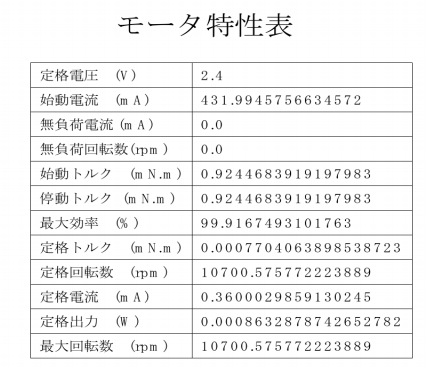
\includegraphics[width=7cm]{./Image/characteristicTable.png}
    }
    \caption{タイトルと特性表の画像}
	\label{fig:toku_gazou}
\end{figure}

\subsection{特性グラフ生成}\label{sub:toku_gurahu}
\ref{sub:csv_scan}節、\ref{sub:youso_kiso}節で求めた要素の配列を用いて、特性グラフを生成する。
処理の流れを以下に示す。
\begin{enumerate}
    % \item 配列torqueに、torque\_defaultを格納する
    % \item 配列currentに、current\_defaultを格納する
    % \item 配列speedに、angularvelocity\_defaultから\ref{siki:speed}式を適用した値を格納する
    % \item current\_defaultが0か判定し、以下の処理を行う
    % \begin{enumerate}
    %     \item 0だった場合、配列efficiencyに、0を格納する
    %     \item 0ではない場合、以下の処理を行う
    %     \begin{enumerate}
    %         \item current\_defaultと、voltage\_defaultを用いて\ref{siki:in}式から、0.0秒段階の入力の値を保持するinput\_defaultに代入する
    %         \item torque\_defaultと、angularvelocity\_defaultを用いて\ref{siki:out}式から、0.0秒段階の出力の値を保持するoutput\_defaultに代入する
    %         \item 配列efficiencyに、input\_defaultと、output\_defaultを\ref{siki:effi}式に適用した値を格納する
    %     \end{enumerate}
    % \item 配列outputに、torque\_defaultと、angularvelocity\_defaultを\ref{siki:out}式に適用した値を格納する
    % \end{enumerate}
    \item x軸に配列torqueを、y軸に配列currentを指定し、ライブラリmatplotlib(表\ref{tab:libr}参照)を用いてグラフを生成し、画像として保存する
    \item 1.の処理に対して、y軸に配列speedを指定した場合、y軸に配列efficiencyを指定した場合、y軸に配列outputを指定した場合を適用し、それぞれグラフを画像として保存する
\end{enumerate}
上記の処理で生成した4つのグラフを、それぞれ図\ref{fig:current}、図\ref{fig:speed}、図\ref{fig:effi}、図\ref{fig:output}に示す。

\begin{figure}[t]
    \begin{tabular}{cc}
        \begin{minipage}{0.45\hsize}
            \centering
            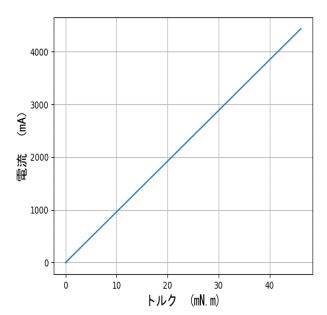
\includegraphics[width=.8\columnwidth]{./Image/current.png}
            \caption{「トルク $\times$ 電流」グラフ}
            \label{fig:current}
        \end{minipage}
        \hfill
        \begin{minipage}{0.45\hsize}
            \centering
            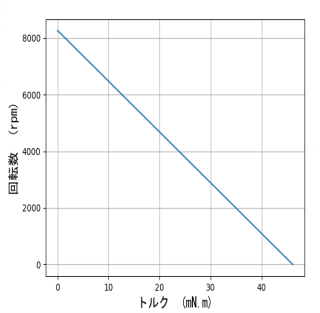
\includegraphics[width=.82\columnwidth]{./Image/speed.png}
            \caption{「トルク $\times$ 回転数」グラフ}
            \label{fig:speed}
        \end{minipage}\\\\
        \begin{minipage}{0.45\hsize}
            \centering
            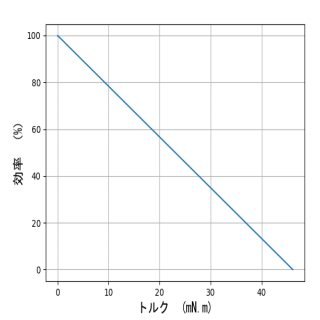
\includegraphics[width=.84\columnwidth]{./Image/efficiency.png}
            \caption{「トルク $\times$ 効率」グラフ}
            \label{fig:effi}
        \end{minipage}
        \hfill
        \begin{minipage}{0.45\hsize}
            \centering
            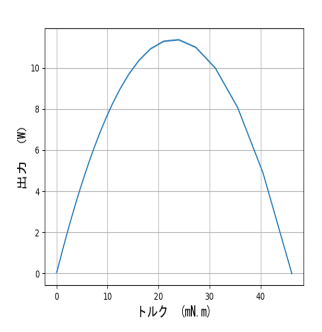
\includegraphics[width=.8\columnwidth]{./Image/output.png}
            \caption{「トルク $\times$ 出力」グラフ}
            \label{fig:output}
        \end{minipage}
    \end{tabular}
\end{figure}
% \begin{figure}[t]
% 	\centering
% 	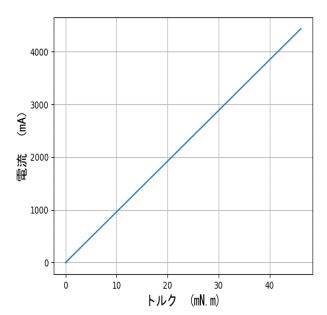
\includegraphics[width=7cm]{./Image/current.png}
% 	\caption{「トルク $\times$ 電流」グラフ}
% 	\label{fig:current}
% \end{figure}
% \begin{figure}[t]
% 	\centering
% 	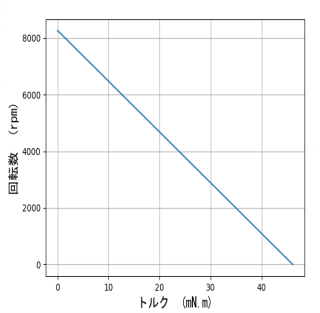
\includegraphics[width=7cm]{./Image/speed.png}
% 	\caption{「トルク $\times$ 回転数」グラフ}
% 	\label{fig:speed}
% \end{figure}
% \begin{figure}[t]
% 	\centering
% 	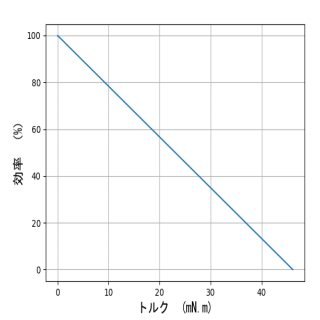
\includegraphics[width=7cm]{./Image/efficiency.png}
% 	\caption{「トルク $\times$ 効率」グラフ}
% 	\label{fig:effi}
% \end{figure}
% \begin{figure}[t]
% 	\centering
% 	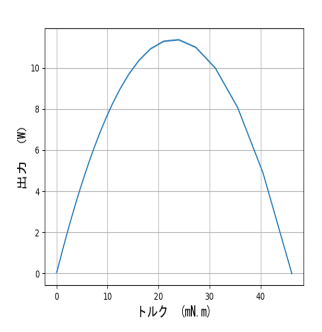
\includegraphics[width=7cm]{./Image/output.png}
% 	\caption{「トルク $\times$ 出力」グラフ}
% 	\label{fig:output}
% \end{figure}
\subsection{モータ特性表生成}\label{sub:a}
\ref{sub:mortortoku}節と、\ref{sub:toku_gurahu}節で生成した合計5つの画像を、ライブラリreportlab(表\ref{tab:libr}参照)を用いて、PDFファイルに書き込み、モータ特性表を生成する。
モータ特性表のPDFファイルのファイル名は、「characteristicTable.pdf」で生成する。同じファイル名のPDFファイルがある場合、上書き保存する。
この処理で生成するモータ特性表を、図\ref{fig:tokuseihyou}に示す。
\begin{figure}[t]
	\centering
	\fbox{
	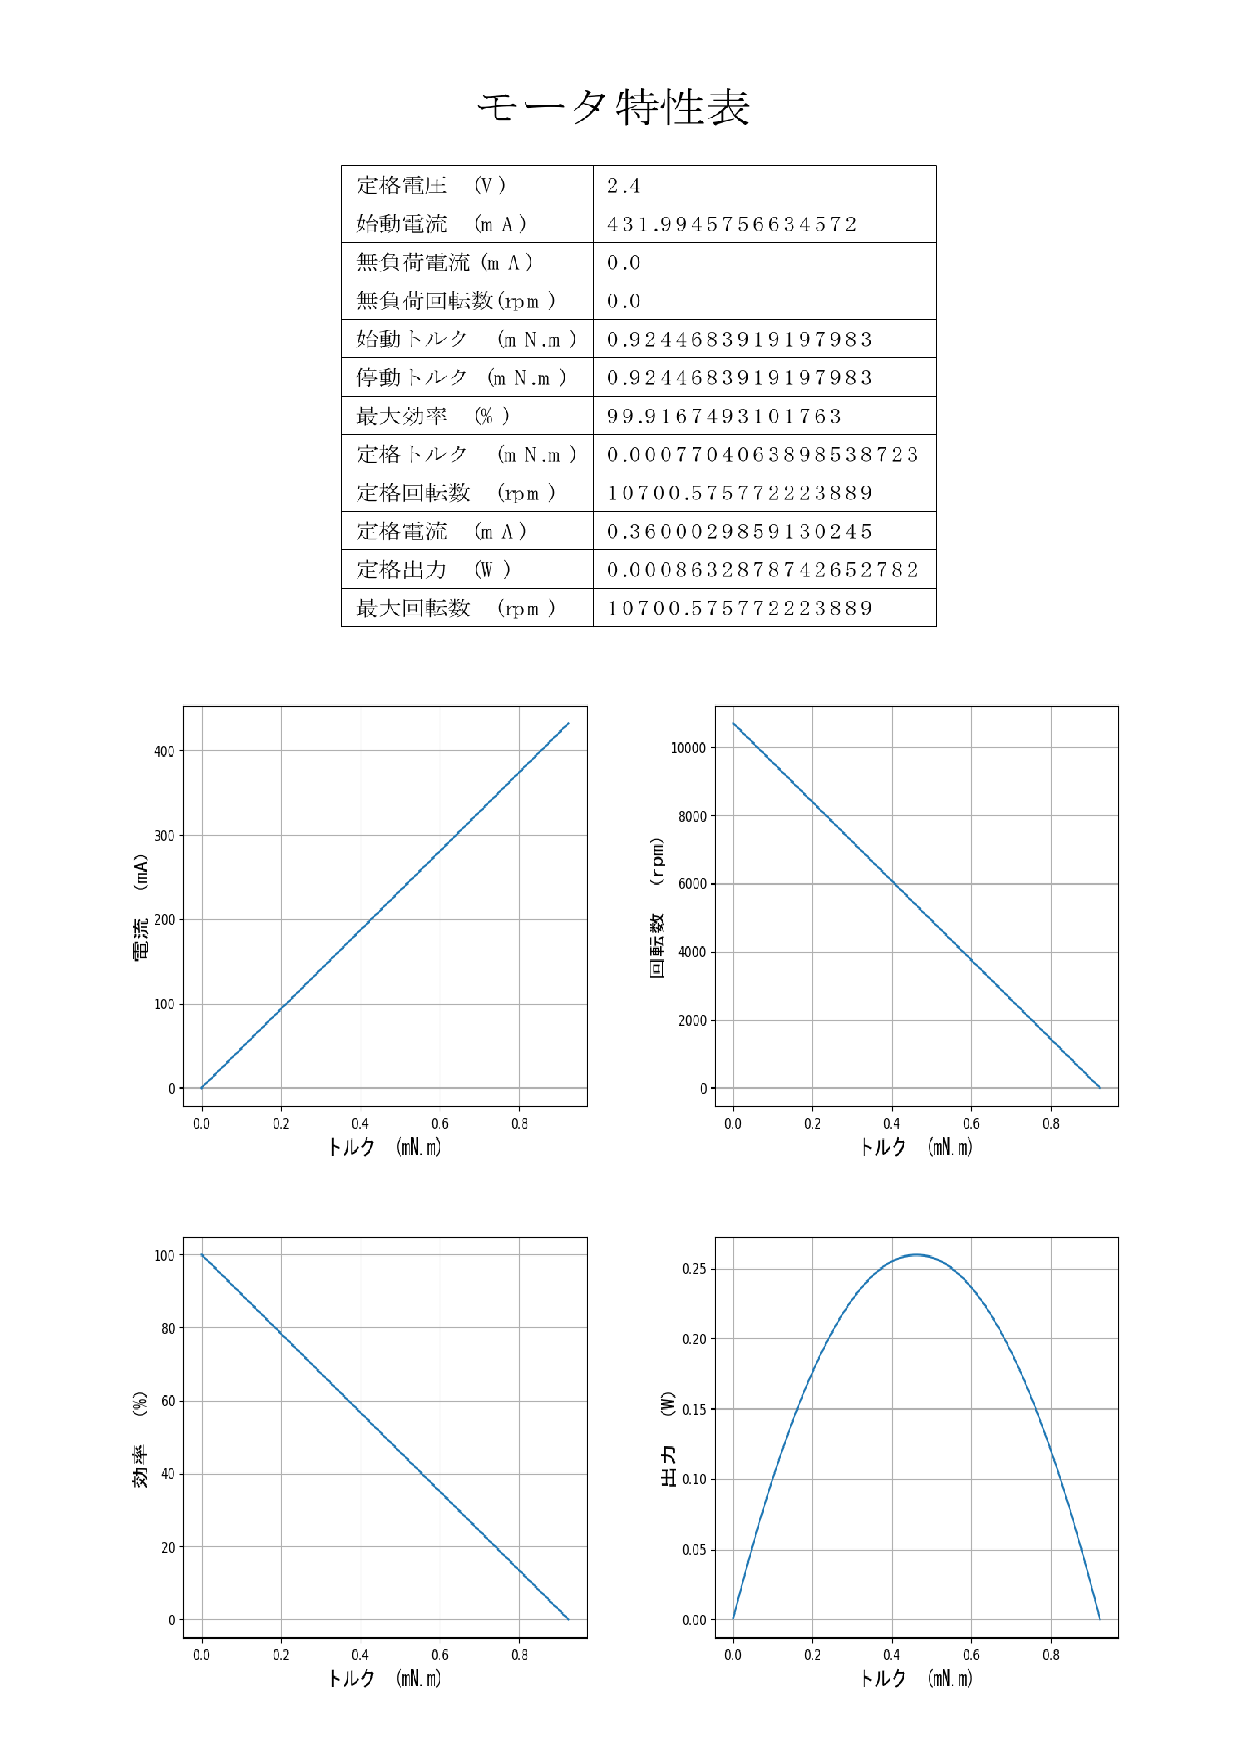
\includegraphics[width=16cm,pagebox=cropbox]{Image/characteristicTable.pdf} 
	}
	\caption{モータ特性表}
	\label{fig:tokuseihyou}
\end{figure}
% \input{chapters/Function.tex}
% \input{chapters/Implementation.tex}
\chapter{適用例}\label{cha:Indication}
% 本章では、本研究で作成したモータ特性表自動生成ツールが正しく動作することを検証するため、以下の同じ能力である2種類のModelicaモデルのシミュレーション結果のcsvファイルを適用する。
本章では、本研究で作成したモータ特性表自動生成ツールが正しく動作することを確認する。
適用例として、ブラシ付きDCモータのModelicaモデルと、
ブラシ付きDCモータのModelicaモデルをサブシステムとするモデルの2つから出力するcsvファイルを適用例として用いる。
また、2つのモータの性能は同じである。
正しく動作しているか確認するために、以下の2つの点に着目する。
% 以下に示す2種類のModelicaモデルのシミュレーション結果のcsvファイルを適用例として用いる。
% 以下のモータは、性能は同じである。
% \begin{itemize}
%     \item ブラシ付きDCモータのModelicaモデル
%     \item ブラシ付きDCモータのModelicaモデルをサブシステムとするモデル
% \end{itemize}

% 2つのモデルのパラメータ設定を以下に示す。
% \begin{itemize}
%     \item 電源部品 ・・・ 9 V
%     \item 抵抗部品 ・・・ 1.78 $\Omega$
%     \item インダクタ部品 ・・・ 0.0000735 H
%     \item 起電力部品 ・・・ 0.010400000000000001 $mN \cdot m$
%     \item 慣性部品 ・・・ 0.00371135959 $\mathrm{kg\cdot m^2}$
% \end{itemize}
% 具体的には、以下の2つの項目を確認する。

\begin{enumerate}
    \item 生成したモータ特性表の各要素の値が、正しい値になっていること
    \item 2つのモデルから生成したモータ特性表の各要素が、同値になっていること
\end{enumerate}


\section{ブラシ付きDCモータのModelicaモデル}
\begin{figure}[t]
	\centering
	\includegraphics[width=10cm]{./Image/tekiyou_tanntai.png}
	\caption{適用するブラシ付きDCモータのModelicaモデル}
	\label{fig:tekiyou_tanntai}
\end{figure}

\begin{figure}[t]
	\centering
	\fbox{
    \includegraphics[width=13cm]{./Image/kakunin_csv.png}
    }
	\caption{図\ref{fig:tekiyou_tanntai}のシミュレーション結果であるcsvファイルの一部}
	\label{fig:tekiyou_csv}
\end{figure}

ブラシ付きDCモータのModelicaモデルをOpenModelicaで実行し、生成されたcsvファイルを、モータ特性表自動生成ツールに適用する。
適用例に用いるモデルを、図\ref{fig:tekiyou_tanntai}に示す。
また、図\ref{fig:tekiyou_tanntai}のシミュレーション結果であるcsvファイルを、図\ref{fig:tekiyou_csv}に示す。
図\ref{fig:tekiyou_csv}のcsvファイルをモータ特性表自動生成ツールに適用した結果、出力するモータ特性表を図\ref{fig:tekiyou_mortoku}に示す。

\begin{figure}[t]
	\centering
	\fbox{
    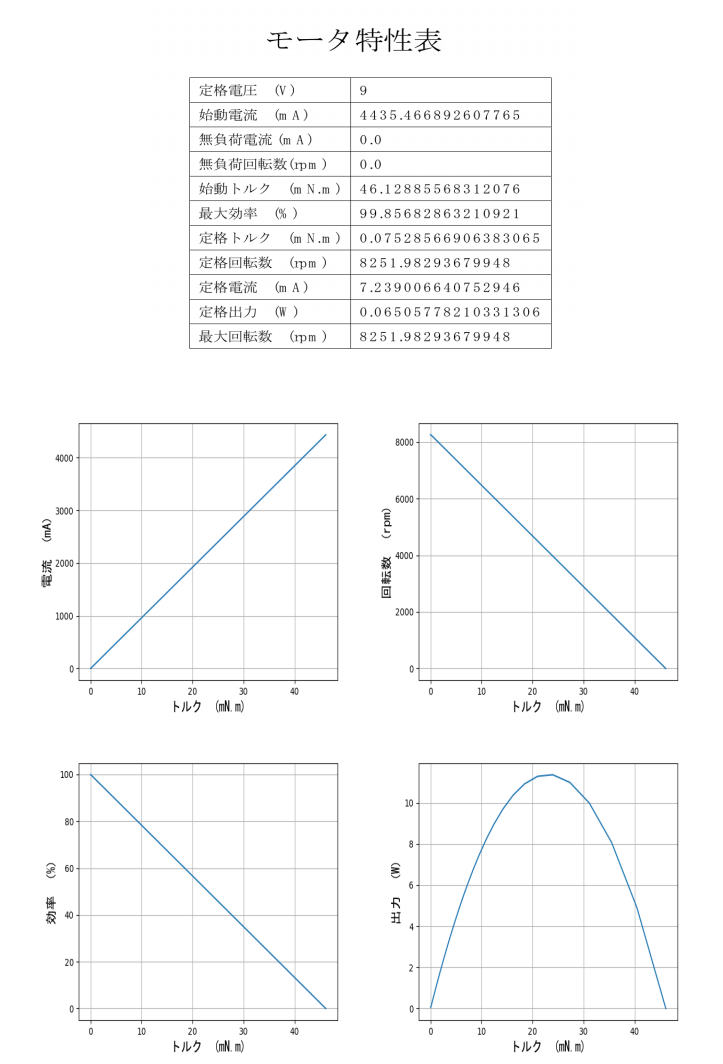
\includegraphics[width=14cm]{./Image/tekiyou_mortoku.png}
    }
    \caption{適用例で生成したモータ特性表}
	\label{fig:tekiyou_mortoku}
\end{figure}
\begin{figure}[t]
	\centering
	\fbox{
    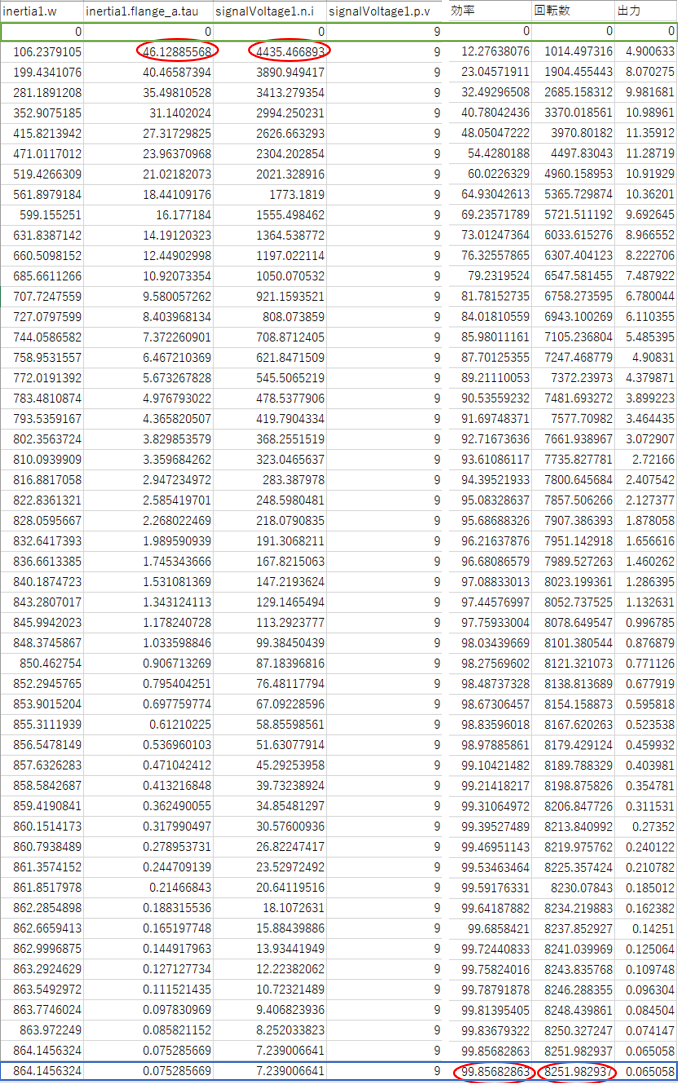
\includegraphics[width=13cm]{./Image/kakunin_saidai_mark.png}
    }
	\caption{図\ref{fig:tekiyou_tanntai}のシミュレーション結果であるcsvファイルの一部と効率と回転数と出力}
	\label{fig:tekiyou_csv_wakariyasui}
\end{figure}

\clearpage

\subsection{特性表の確認}
図\ref{fig:tekiyou_tanntai}のシミュレーション結果であるcsvファイルからモータ特性表を作成する際に使用する要素を、
図\ref{fig:tekiyou_csv_wakariyasui}に示す。
図\ref{fig:tekiyou_csv_wakariyasui}の赤丸は最大値を、青色の四角形は最大効率時の行を、緑色の四角形は無負荷時の行を表す。

出力した特性表の各要素が正しく算出できているか確認した結果を、以下に示す。
%図\ref{fig:kakunin_csv}には、図\ref{fig:tekiyou_csv}から効率と回転数を算出したデータを示す。図中の赤丸は最大値を、青い四角形は最大効率時の行を表す。
% \begin{figure}[t]
% 	\centering
% 	\fbox{
%     \includegraphics[width=3cm]{./Image/tekiyou_csv_kakunin.png}
%     }
%     \caption{図\ref{fig:tekiyou_csv}から効率と回転数を算出}
% 	\label{fig:kakunin_csv}
% \end{figure}

\subsubsection{定格電圧}
図\ref{fig:tekiyou_mortoku}の特性表にある定格電圧の値と、
図\ref{fig:tekiyou_csv_wakariyasui}のsignalVoltage1.p.vが持つ値の中で、先頭にある値が同値である。
したがって、正しく出力していることが確認できる。

\subsubsection{始動電流}
図\ref{fig:tekiyou_mortoku}の特性表にある始動電流の値と、
図\ref{fig:tekiyou_csv_wakariyasui}のsignalVoltage1.n.iが持つ値の中の最大値が同値である。
したがって、正しく出力していることが確認できる。


\subsubsection{無負荷電流}
図\ref{fig:tekiyou_mortoku}の特性表にある無負荷電流の値と、
図\ref{fig:tekiyou_csv_wakariyasui}のsignalVoltage1.n.iが持つ値の中の
無負荷を出した時の値が同値である。

\subsubsection{無負荷回転数}
図\ref{fig:tekiyou_mortoku}の特性表にある無負荷回転数の値と、
図\ref{fig:tekiyou_csv_wakariyasui}の回転数が持つ値の中の
無負荷を出した時の値が同値である。


\subsubsection{停動トルク}
図\ref{fig:tekiyou_mortoku}の特性表にある停動トルクの値と、
図\ref{fig:tekiyou_csv_wakariyasui}のinertia1.flange\_a.tauが持つ値の中の最大値が同値である。
したがって、正しく出力していることが確認できる。

\subsubsection{最大効率}
図\ref{fig:tekiyou_mortoku}の特性表にある最大効率の値と、
図\ref{fig:tekiyou_csv_wakariyasui}の効率が持つ値の中の最大値が同値である。
したがって、正しく出力していることが確認できる。

\subsubsection{定格トルク}
図\ref{fig:tekiyou_mortoku}の特性表にある定格トルクの値と、
図\ref{fig:tekiyou_csv_wakariyasui}のinertia1.flange\_a.tauが持つ値の中の、最大効率を出した時の値が同値である。
したがって、正しく出力していることが確認できる。

\subsubsection{定格回転数}
図\ref{fig:tekiyou_mortoku}の特性表にある定格回転数の値と、
図\ref{fig:tekiyou_csv_wakariyasui}の回転数が持つ値の中の、最大効率を出した時の値が同値である。
したがって、正しく出力していることが確認できる。

\subsubsection{定格電流}
図\ref{fig:tekiyou_mortoku}の特性表にある定格電流と、
図\ref{fig:tekiyou_csv_wakariyasui}のsignalVoltage1.n.iが持つ値の中の、
最大効率を出した時の値が同値である。
したがって、正しく出力していることが確認できる。

\subsubsection{定格出力}
% 出力は、\mbox{ トルク $(\mathrm{N \cdot m})$} $\times$ \mbox{角速度 $(\mathrm{rad/s})$} で算出することが可能である。
図\ref{fig:tekiyou_mortoku}の特性表にある定格出力と、
図\ref{fig:tekiyou_csv_wakariyasui}の出力が持つ値の中の、最大効率を出した時の値が同値である。
したがって、正しく出力していることが確認できる。

% 図\ref{fig:tekiyou_mortoku}の特性表にある出力と、図\ref{fig:tekiyou_csv}の最大効率時のinertia1.flange\_a.tauが持つ値と、inertia1.flange\_a.wが持つ値を(\ref{siki:speed})式に適用した結果が同値である。
% よって、正しく出力していることが確認できる。
\subsubsection{最大回転数}
図\ref{fig:tekiyou_mortoku}の特性表にある最大回転数と、
図\ref{fig:tekiyou_csv_wakariyasui}の回転数が持つ値の中の最大値が同値である。
したがって、正しく出力していることが確認できる。

\subsection{特性グラフの確認}
出力した特性グラフが正しく算出できているか確認した結果を、以下に示す。

\subsubsection{「トルク $\times$ 電流」グラフ}
図\ref{fig:tekiyou_mortoku}の特性グラフにある「トルク $\times$ 電流」グラフに、
図\ref{fig:tekiyou_csv}のinertia1.flange\_a.tauが持つ値と、
signalVoltage1.n.iが持つ値が存在するので、正しく生成していることが確認できる。

\subsubsection{「トルク $\times$ 回転数」グラフ}
図\ref{fig:tekiyou_mortoku}の特性グラフにある「トルク $\times$ 回転数」グラフに、
図\ref{fig:tekiyou_csv}のinertia1.flange\_a.tauが持つ値と、
回転数が持つ値が存在するので、正しく生成していることが確認できる。

\subsubsection{「トルク $\times$ 効率」グラフ}
図\ref{fig:tekiyou_mortoku}の特性グラフにある「トルク $\times$ 効率」グラフに、
図\ref{fig:tekiyou_csv}のinertia1.flange\_a.tauが持つ値と、
図\ref{fig:sub_mortoku}の効率が持つ値が存在するので、正しく生成していることが確認できる。

\subsubsection{「トルク $\times$ 出力」グラフ}
図\ref{fig:tekiyou_mortoku}の特性グラフにある「トルク $\times$ 出力」グラフに、
図\ref{fig:tekiyou_csv}のinertia1.flange\_a.tauが持つ値と、
図\ref{fig:sub_mortoku}の出力が持つ値が存在するので、正しく生成していることが確認できる。


\section{ブラシ付きDCモータのModelicaモデルをサブシステムとするモデル}
今回適用するブラシ付きDCモータのModelicaモデルをサブシステムとするモデルは、
図\ref{fig:tekiyou_tanntai}のモデルと同じ性能になるよう設計する。
そして、どちらのモータ特性表も同じ内容であることを確認する。

今回適用するブラシ付きDCモータのModelicaモデルをサブシステムとするモデルを、
図\ref{fig:tekiyou_sub}に、図\ref{fig:sub_mortoku}の生成したモータ特性表を、図\ref{fig:sub_mortoku}にそれぞれ示す。

\begin{figure}[t]
	\centering
	\includegraphics[width=10cm]{./Image/tekiyou_sub.png}
	\caption{適用するブラシ付きDCモータのModelicaモデルをサブシステムとするモデル}
	\label{fig:tekiyou_sub}
\end{figure}

\begin{figure}[t]
	\centering
	\fbox{
	\includegraphics[width=16cm,pagebox=cropbox]{Image/characteristicTable_kakunin.pdf}
	}
	\caption{図\ref{fig:tekiyou_sub}のモデルを基に生成したモータ特性表}
	\label{fig:sub_mortoku}
\end{figure}

図\ref{fig:tekiyou_mortoku}と図\ref{fig:sub_mortoku}の内容が同じであるため、生成した2つのモータ特性表に共通する各要素が、同値であることが確認できる。

% \todo{おわりにで書く:『よって、モータ特性表自動生成ツールは、「ブラシ付きDCモータのModelicaモデル」と「ブラシ付きDCモータのModelicaモデルをサブシステムとするモデル」に対応していることが確認できる。』}

\chapter{考察}\label{cha:Discussion}
本論文では、性能を決定付ける特定の値を確認するためにかかる時間の削減を目的として、OpenModelicaのシミュレーション結果を用いたモータ特性表自動生成ツールを試作した。

なお、本研究では、シミュレーションの対象として、ブラシ付きDCモータのみとする。

4章において、本論文で試作したモータ特性表自動生成ツールに、ブラシ付きDCモータのModelicaモデルから出力するcsvファイルを適用した。
その結果、本論文で試作したモータ特性表自動生成ツールが正しく動作することを確認できた。以下に、本論文で試作したモータ特性表自動生成ツールについて考察する。
\section{ツールの有用性評価}

\subsection{評価方法}
% \todo{下記のコマンドを書き換える!}
% \newcommand{\mExist}{既存の手法}
% \newcommand{\mExtend}{本研究の手法}
% \newcommand{\mInput}{仕様書}
% \newcommand{\mOutput}{仕様書}

% \mExist{}と、\mExtend{}で、作成(生成)に要した時間の比較検証を行った。
% その結果を、表\ref{tab:time}に示す。

% 対象とした\mInput{}は、\ref{cha:domain}節で用いた コード\ref{fig:vdm_park}である。
% \mOutput{}を作成する時間を計測した。
% 生成する\mOutput{}としては、以下を基準とした。\todo{なにをもって完成かを書く!}
% \begin{enumerate}
%   \item onポイント、offポイント、inポイント、outポイントを出力(記述)する
%   \item onポイント、offポイント、outポイントには、着目条件式も出力(記述)する
%   \item offポイントには、着目変数も出力(記述)する
%   \item 各ポイントには、期待出力と正常系であるかどうかも出力(記述)する
% \end{enumerate}

% 検証に参加したメンバーは本研究室の大学院生\todo{X}人と学部4年生\todo{Y}人であり、
% 普段からソースコードの読み書きを行い、基本的なプログラミングの知識を有している。
% \mInput{}の知識を持たない者も含まれるが、
% 今回の検証に必要な文法は、事前に他の\mInput{}の例を用いてレクチャーした。
% また、\mOutput{}生成についても、事前に他の\mInput{}と\mOutput{}の例を用いてレクチャーした。

% 人手による検証では、
% コード\ref{fig:vdm_park}を印刷した紙を渡し、
% \mInput{}を確認後、
% \mOutput{}を書き始めてから、\mOutput{}を記述し終えるのに要した時間を計測した。
% \todo{なんか}が不正確な場合、間違いを指摘し、
% 被験者が正しい\mOutput{}を記述した時点で時間計測終了とした。
% また、制限時間を\todo{Z}分とし、制限時間を超えた場合、その場で時間計測終了とした。

% \mExtend{}による検証では、
% \todo{計測はじめから終わりの条件と、使ったPCの仕様を書く}
% コマンドライン上での命令操作で、\mExtend{}による\mOutput{}生成を行うのに要した時間を計測した。
% また、実験に用いたコンピュータは、OS:Windows10 Pro、CPU:3.6GHz Intel Core i7、メモリ:16GBである。

% \todo{純粋な、実行時間を書く}
% なお、JavaのSystem.nanoTime\cite{nanotime}メソッドを用いて、
% 命令操作を省いた純粋な\mOutput{}生成処理に\mExtend{}が要した時間を計測した結果、
% \todo{A}秒であった。

% 人手による作成と比較した結果、平均で\todo{B}分程の時間短縮を確認できた。
% 対象にした\mInput{}には、\todo{なにか}独特の文法等は含まれないため、
% \todo{なにか}に対する慣れなどの影響は無視できるものと思われる。
% また、人手による\mOutput{}生成の場合、ヒューマンエラーも見られた。
% \todo{ヒューマンエラーがあったら、具体例を書く}
% 具体的には、offポイントの記述時に、条件式の解釈を間違え、誤った期待出力を記述してしまった。(例:入力(17、 20)の期待出力を``遊園地チケットは割引価格とならない。(妻の年齢 $<$ 16)''と記述した。)
% \mInput{}の規模が拡大すると、人手とコンピュータとの処理効率の差に加えて、
% ヒューマンエラーの有無などにより、\mOutput{}生成に要する時間の差は更に拡大していくと思われる。
% 以上から、\mExtend{}は有用性が向上したと考える。

% % \begin{table}[tp]
% % \centering
% % \caption{コード\ref{fig:vdm_park}の\mOutput{}作成に要した時間の比較}
% % \label{tab:time}
% % \begin{tabular}{cc}
% % \begin{minipage}[c]{0.5\hsize}
% %   \centering
% %   \begin{tabular}{c|c}
% %     被験者  & 時間              \\
% %     \hline
% %     \hline
% %     被験者A & 8m 16s            \\ \hline
% %     被験者B & 10m 23s           \\ \hline
% %     被験者C & 30m(制限時間超過) \\ \hline
% %     被験者D & 24m 04s
% %   \end{tabular}
% % \end{minipage} &
% % \begin{minipage}[c]{0.5\hsize}
% %   \centering
% %   \begin{tabular}{c|c}
% %                  & 時間    \\
% %     \hline
% %     \hline
% %     被験者(平均) & 18m 10s \\ \hline
% %     BWDM         & 0m 15s
% %   \end{tabular}
% % \end{minipage}
% % \end {tabular}
% % \end{table}

本論文で試作したモータ特性表自動生成ツールの有用性を評価するため、本研究室の学部4年生4人に対して、実験を行い、特定の値を確認するためにかかる時間を削減できたかどうかを検証する。
実験には、内容が異なる2つのシミュレーション結果のファイルを用いた。これらのファイルをそれぞれファイルA、ファイルBと定義する。

実験方法は、ケースXとケースYに分けて行う。

ケースXでは、ファイルAに対して、モータ特性表自動生成ツールを使用せず、表計算ソフトを用いて問題に回答してもらう。次に、ファイルBに対して、モータ特性表自動生成ツールを使用して問題に回答してもらう。

ケースYでは、ファイルBに対して、モータ特性表自動生成ツールを使用せず、表計算ソフトを用いて問題に回答してもらう。次に、ファイルAに対して、モータ特性表自動生成ツールを使用して問題に回答してもらう。

ケースXとケースY で出題する問題を、図\ref{fig:mondai}に示す。

この問題を解答するのに要する時間を測定することにより、モータ特性表自動生成ツールを用いることで、特定の値を確認するためにかかる時間を削減できるかどうかを検証する。

被験者4名を2つのグループに分け、片方のグループにケースXの実験を行い、もう片方のグループにケースYの実験を行った。

ケースXの実験結果を表\ref{resultX}に、ケースYの実験結果を表\ref{resultY}に、それぞれ示す。

\begin{figure}[t]
	\centering
	\fbox{
	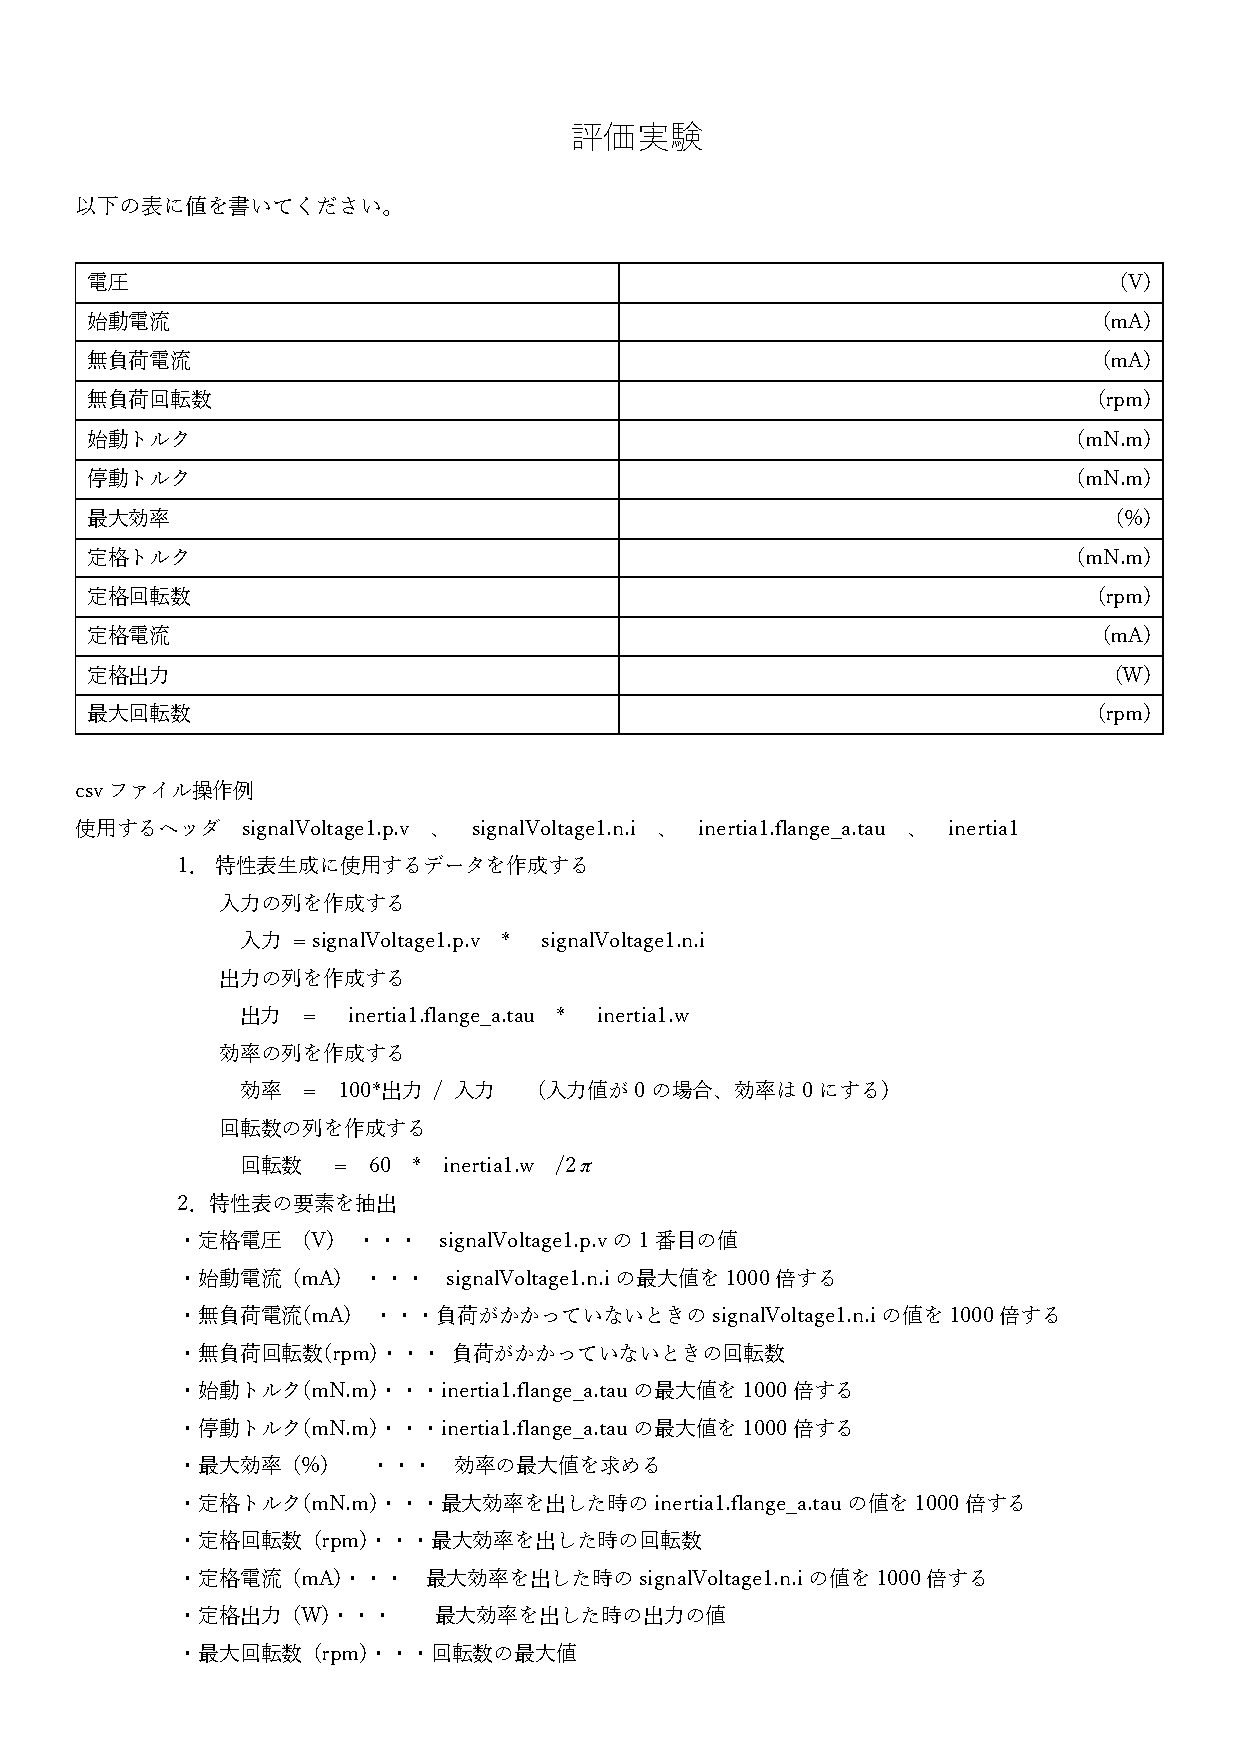
\includegraphics[width=16cm,pagebox=cropbox]{Image/実験方法の説明.pdf}
	}
	\caption{ケースXとケースY で出題する問題}
	\label{fig:mondai}
\end{figure}
\clearpage
\begin{table}[tp]
  \begin{center}
    \caption{ケースXの実験結果}
    \label{resultX}
    \begin{tabular}{c|c|c|c|c|}
    \cline{2-5}
                              & \multicolumn{2}{c|}{ツール未使用} & \multicolumn{2}{c|}{ツール使用} \\ \hline
    \multicolumn{1}{|c||}{被験者} & 回答時間           & 正答率          & 回答時間           & 正答率         \\ \hline\hline
    \multicolumn{1}{|c||}{1}   & 13分5秒           & 56\%         & 57秒           & 100\%         \\ \hline
    \multicolumn{1}{|c||}{2}   & 14分50秒          & 67\%          & 1分20秒          & 100\%         \\ \hline\hline
    \multicolumn{1}{|c||}{平均}   & 13分57.5秒          & 61.5\%          & 1分8.5秒          & 100\%         \\ \hline
    \end{tabular}
  \end{center}
\end{table}

\begin{table}[tp]
  \begin{center}
    \caption{ケースYの実験結果}
    \label{resultY}
    \begin{tabular}{c|c|c|c|c|}
    \cline{2-5}
                              & \multicolumn{2}{c|}{ツール未使用} & \multicolumn{2}{c|}{ツール使用} \\ \hline
    \multicolumn{1}{|c||}{被験者} & 回答時間           & 正答率          & 回答時間           & 正答率         \\ \hline\hline
    \multicolumn{1}{|c||}{3}   & 21分35秒           & 67\%         & 1分10秒           & 100\%         \\ \hline
    \multicolumn{1}{|c||}{4}   & 18分6秒          & 100\%          & 1分58秒          & 89\%         \\ \hline\hline
    \multicolumn{1}{|c||}{平均}   & 19分50.5秒          & 83.5\%          & 1分34秒          & 94.5\%         \\ \hline
    \end{tabular}
  \end{center}
\end{table}

ケースXの実験結果から、モータ特性表自動生成ツールを用いない場合の解答時間の平均は13分57.5秒である。また、正答率の平均は61.5\%である。
一方、モータ特性表自動生成ツールを用いた場合の解答時間の平均は1分8.5秒である。また、正答率の平均は100\%である。

この結果から、ケースXの実験においてモータ特性表自動生成ツールを用いた場合、解答時間の平均は用いなかった場合に比べて91.8\%削減できた。
また、モータ特性表自動生成ツールを用いた場合の方が、用いなかった場合に比べて正答率が高いことが示せた。

ケースYの実験結果から、モータ特性表自動生成ツールを用いない場合の解答時間の平均は19分50.5秒である。また、正答率の平均は83.5\%である。
一方、モータ特性表自動生成ツールを用いた場合の解答時間の平均は1分34秒である。また、正答率の平均は94.5\%である。
なお、被験者4は自動生成したモータ特性表の値の確認を誤ったため、正答率が89\%となった。

この結果から、ケースYの実験においてモータ特性表自動生成ツールを用いた場合、解答時間の平均は用いなかった場合に比べて92.1\%削減できた。
また、モータ特性表自動生成ツールを用いた場合の方が、用いなかった場合に比べて正答率が高いことが示せた。


これらの実験結果より、モータ特性表自動生成ツールを用いた場合は、用いなかった場合に比べて、
解答に要する時間を平均で、91.95\%削減できた。また、モータ特性表自動生成ツールを用いた場合が、用いなかった場合に比べて正答率が高いことを示せた。正答率が上がった理由として、
モータ特性表自動生成ツールを用いることにより、人手によるミスを削減できたことが考えられる。
具体的には、モータ特性表自動生成ツールを用いない場合、手動で表計算ソフトから特定の値を抽出し、計算を行う必要があるため、この過程においてミスが発生する可能性が高かったことが考えられる。
一方、モータ特性表自動生成ツールを用いた場合、ツールが自動で特性表を生成し、指定の値を提示することにより、人手によるミスが発生する可能性を削減できたことが考えられる。

以上の結果により、モータ特性表自動生成ツールの有用性があることを示せた。また、モータ特性表自動生成ツールを用いることで、特定の値を確認する際に生じるミスを削減できることが確認できた。

\section{関連研究}
関連研究について考察する。

\subsection{MATLABとの比較}
モデルベースシステム開発で使用されるツールとして、OpenModelicaの他に、MATLAB\cite{MATLAB技術30:online}がある。
MATLABはMathWorks社が開発する科学技術計算用のプログラミング言語である。
MATLABは、制御システム、信号処理、ディープラーニングなど幅広い分野の科学技術計算ができる。
また、ブロック線図シミュレータであるSimulink\cite{Simulink81:online}と連携させることで、モータのモデル化、シミュレーション、グラフの描画ができる。
しかし、モータの性能を決定づける値の算出や、グラフの描画はできるが、モータ特性表を自動生成できない。
一方、本研究で試作したモータ特性表自動生成ツールは、OpenModelicaのシミュレーション結果から、モータ特性表を自動生成できる。
このため、特性表と特性グラフをまとめたモータ特性表を自動生成できることが試作したツールの利点といえる。


\subsection{JMAG-Express Onlineとの比較}
\begin{table}[t]
	\centering
	\caption{本研究で試作したモータ特性表自動生成ツールにおけるモータ特性表を出力するまでの実行時間}
	\begin{tabular}{|c|c|} \hline
	  ファイルサイズ(KB) & 実行時間(s)\\ \hline \hline
	  37 & 0.884 \\ \hline
	  47 &  0.978\\ \hline
	  2,909 &  1.024 \\ \hline
	  3,569 & 1.025 \\ \hline
	  5,496 &  1.078\\ \hline
	  71,987 &  3.329 \\ \hline
	\end{tabular}
	\label{tab:executionTime}
  \end{table}

パラメータベースのモータ設計支援ツールとして、JSOL社が開発するJMAG-Express Online(以下JMAG)がある\cite{jmag}。
JMAGは、形状テンプレート、材料、巻線および駆動条件のパラメータを入力することで、
モータ特性表を生成することができる。
さらに、モータ特性表に出力する基本特性(トルク、回転数など)は1秒程度で計算できる。
しかし、パラメータベースのモータ設計支援ツールであるため、
モデルベースシステム開発の利点である「製品の設計を元にシミュレーションツールを用いて、シミュレーションを行いながら、設計品質の向上を図る」開発において、JMAGを利用できない。
一方、本研究で試作したモータ特性表自動生成ツールは、OpenModelicaのシミュレーション結果から、
モータ特性表を自動生成できる。
ここで、本研究で試作したモータ特性表自動生成ツールにおけるモータ特性表を出力するまでの実行時間を、表\ref{tab:executionTime}に示す。
表\ref{tab:executionTime}が示すように、試作したツールも1秒程度でモータ特性表に出力する基本特性を計算できるため、JMAGと同程度の時間で、モータ特性表を生成できる。
このため、モータをモデルベースシステム開発手法で開発する際に、試作したツールを用いてモータの性能を確認できることが、試作したツールの利点といえる。
また、実験に用いたコンピュータは、OS:Windows10 Pro、CPU:3.6GHz Intel Core i7、メモリ:16GBである。

\section{ツールの問題点}

以下に、今回作成したモータ特性表自動生成ツールの問題点を示す。

% \begin{itemize}
% 	\item 対象とするモータのモデルが1種類しかない\\
%       本論文で試作したモータ特性表自動生成ツールが対象とするのはブラシ付きDCモータである。しかし、ブラシレスモータやACモータなどには対応していない。
%       そのため、それらを用いた回路のシミュレーション結果からモータ特性表を作成できない。
% 		  この問題点は、新たに対象とするモータのcsvファイルを解析し、特性表の要素を算出できるようにすることで、解決できると考える。

%   \item 特性表の要素をユーザが変更できない\\
%         本論文で試作したモータ特性表自動生成ツールが生成する特性表は、12個の要素を持つ。
%         しかし、ユーザがこの要素を変更することはできない。
%         この問題点は、ユーザが特性表の要素を設定できるようにすることで、解決できると考える。

%   \item 特性グラフを出力形式をユーザが指定できない\\
%         本論文で試作したモータ特性表自動生成ツールは、4つの特性グラフを個別に出力する。
%         しかし、特性グラフは1つのグラフに複数の要素を表示することで、グラフの比較を行いやすくなる。
%         そのため、特性グラフの出力形式をユーザが指定できるようにすることで、グラフの比較がしやすくなり、 本論文で試作したモータ特性表自動生成ツールの有用性が向上すると考える。

\begin{itemize}
  % \setlength{\itemsep}{0pt}
  \item 対象とするモータのモデルの拡大\\
    本論文で試作したモータ特性表自動生成ツールが対象とするのはブラシ付きDCモータである。しかし、ブラシレスモータやACモータなどには対応していない。
    そのため、それらを用いた回路のシミュレーション結果からモータ特性表を作成できない。
    この問題点は、新たに対象とするモータのcsvファイルを解析し、特性表の要素を算出できるようにすることで、解決できると考える。

\item 特性表の要素のカスタマイズ機能の実装\\
本論文で試作したモータ特性表自動生成ツールが生成する特性表は、12個の要素を持つ。
  しかし、ユーザがこの要素を変更することはできない。
  この問題点は、ユーザが特性表の要素を設定できるようにすることで、解決できると考える。


  \item サブシステムを用いたモデルに対応\\
  本論文で試作したモータ特性表自動生成ツールが対象にするモデルに、サブシステムを用いたモデルは含まれていない。
  サブシステムを用いる場合、そのサブシステムを識別できるように新たに引数を指定し、そのサブモデルの状況を判断できるようにすることで、解決できると考える。  

\item 特性グラフの出力形式のカスタマイズ機能の実装\\
本論文で試作したモータ特性表自動生成ツールは、4つの特性グラフを個別に出力する。
しかし、特性グラフは1つのグラフに複数の要素を表示することで、グラフの比較を行いやすくなる。
そのため、特性グラフの出力形式をユーザが指定できるようにすることで、グラフの比較がしやすくな
り、 本論文で試作したモータ特性表自動生成ツールの有用性が向上すると考える。


\end{itemize}








\chapter{おわりに}\label{cha:Conclusion}
本論文では、性能を決定付ける特定の値を確認するためにかかる時間の削減を目的として、OpenModelicaのシミュレーション結果を用いたモータ特性表自動生成ツールを試作した。
なお、本研究では、シミュレーションの対象として、ブラシ付きDCモータを対象とする。

モータ特性表自動生成ツールは、csvファイル解析部、特性表の要素算出部、モータ特性表生成部の3つの処理部で構成している。
csvファイル解析部では、csvファイルを読み込み、モータ特性表を生成するために必要なデータを抽出する。特性表の要素算出部では、抽出したデータからモータ特性表の各要素を算出する。
モータ特性表生成部では、算出した各要素を基に、特性表と4つの特性グラフを生成し、これらを1つのPDFファイルにまとめ、モータ特性表として出力する。

適用例として、ブラシ付きDCモータのModelicaモデルのシミュレーション結果であるcsvファイルを用いる。このcsvファイルをモータ特性表自動生成ツールに適用した結果、
モータ特性表を正しく生成することを確認した。
% よって、モータ特性表自動生成ツールは、「ブラシ付きDCモータのModelicaモデル」と「ブラシ付きDCモータのModelicaモデルをサブシステムとするモデル」に対応していることが確認できる。

考察において、モータ特性表自動生成ツールの有用性を示すことができた。具体的には、モータ特性表自動生成ツールを用いることにより、特定の値を確認するためにかかる時間を削減できることを検証した。
検証にはケースXとケースYの2種類のケースを用意し、被験者4名を2グループに分けて、モータ特性表自動生成ツールを用いる場合と、用いない場合で実験を行った。

この実験結果により、モータ特性表自動生成ツールを使用した場合では、使用しなかった場合に比べて被験者の解答時間を92.0\%削減できた。
% ケースYについては、モータ特性表自動生成ツールを使用した場合では、使用しなかった場合に比べて被験者の回答時間を92.1\%削減できた。
この結果により、特定の値を確認するためにかかる時間を削減できたと言える。また、双方のケースでモータ特性表自動生成ツールを用いた場合は、モータ特性表自動生成ツールを用いない場合に比べて、正答率が高かった。
% 正答率が上がった理由として、モータ特性表自動生成ツールを用いる
% 人手によるミスを削減できたことが考えられる。具体的には、モータ特性表自動生成ツールを用いない場合、手動で表計算ソフトから特定の値を抽出し、計算を行う必要があるため、
% この過程においてミスが発生する可能性が高まったことが考えられる。
% 一方、モータ特性表自動生成ツールを用いた場合、ツールが自動で特性表を生成し、提示することにより、人手によるミスが発生する可能性を削減できたことが考えられる。

以上の結果により、モータ特性表自動生成ツールの有用性があることを示せた。また、モータ特性表自動生成ツールを用いることで、特定の値を確認する際に生じるミスを削減できることが確認できた。

以下に、今後の課題を示す。

\begin{itemize}
    \item 対象とするモータのモデルの拡大\\
    本論文で試作したモータ特性表自動生成ツールが対象とするのはブラシ付きDCモータである。しかし、ブラシレスモータやACモータなどには対応していない。
    そのため、それらを用いた回路のシミュレーション結果からモータ特性表を作成できない。
    この問題点は、新たに対象とするモータのcsvファイルを解析し、特性表の要素を算出できるようにすることで、解決できると考える。

\item 特性表の要素のカスタマイズ機能の実装\\
      本論文で試作したモータ特性表自動生成ツールが生成する特性表は、12個の要素を持つ。
      しかし、ユーザがこの要素を変更することはできない。
      この問題点は、ユーザが特性表の要素を設定できるようにすることで、解決できると考える。

% \item 特性グラフを出力形式をユーザが指定できない\\
%       本論文で試作したモータ特性表自動生成ツールは、4つの特性グラフを個別に出力する。
%       しかし、特性グラフは1つのグラフに複数の要素を表示することで、グラフの比較を行いやすくなる。


\end{itemize}




\input{listings-modelica.cfg}
%%
% 謝辞
%
\acknowledgment
謝辞を書く

%%
% 参考文献
%

\bibliography{bibtex} %bibファイルの.bibの前の部分


\bibliographystyle{junsrt} %引用された順番に出力

% \newpage
% \listoftodos
\end{document}